\documentclass{article}

\usepackage[margin=2.5cm,left=2cm,includefoot]{geometry}
\usepackage{graphicx}
\usepackage{float}
\usepackage[space]{grffile}
\usepackage{hyperref}
\usepackage[export]{adjustbox}

% Header and footer
\usepackage{fancyhdr}
\pagestyle{fancy}

\rhead{COS301 - \LaTeX}
\lhead{Team Charlie}
\fancyfoot{}
\fancyfoot[R]{Page \thepage}

\renewcommand{\headrulewidth}{2pt}
\renewcommand{\footrulewidth}{1pt}
%

\begin{document}

	\begin{titlepage}
		\begin{center}
		
			\line(1,0){300}\\
			[6mm]
			\huge{
				\bfseries Software Requirements Specification\\
				and\\
				Technology Neutral Process Design
			}\\
			[2mm]
			\line(1,0){200}\\
			[15mm]
			\textsc{\large P.A.P.E.R.S (Publication And Papers Electronic Repository System)}\\
			[7.5mm]
			\textsc{\large University of Pretoria - Team Charlie}\\
			[20mm]
			\large{\textbf{Created By:}}\\
			[2mm]
			\large{
				Claudio Da Silva - 14205892\\
				Arno Grobler - 14011396\\
				Dillon Heins - 14035538\\
				Charl Jansen Van Vuuren - 13054903\\
				Priscilla Madigoe - 13049128\\
				Bernhard Schuld - 10297902\\
				Keorapetse Shiko - 12231992
			}\\
			[4cm]

		\href{https://github.com/DillonHeins/Charlie}{\textsc{\Large GitHub Repository - Team Charlie}\\[2mm]
		  For more information, please click here}
			
		\end{center}	
		\begin{flushright}
			\textsc{\large 17 February 2016}
		\end{flushright}
	\end{titlepage}
	
	\cleardoublepage
	\thispagestyle{empty}
	\tableofcontents
	\cleardoublepage
	\listoffigures
	\cleardoublepage
	\setcounter{page}{1}
	\section{Introduction}\label{sec:intro}
	P.A.P.E.R.S (Publication and Papers Electronic Repository System), a project proposed by the University of Pretoria’s department of Computer Science, is a interdepartmental system dedicated to the management of the research and publication records of each user of the system. The objective of the system is to create an environment where users of the system can maintain a list of publications belonging to them and where supervisors, such as a research leader or head of department, could oversea progress of said users. Users can belong to research groups and maintain a record of who contributed to a publication and thus will consequently affect the unit score each user has. Only members of the department of Computer Science can be users of the system. 
	\subsection{General Uses}\label{subsec:generaluses}
		General uses of this system should include keeping track of:
            \begin{itemize}  
            
                \item Research Papers and publications created by users of the system.
                \item Reporting.
                \item Research Groups.
                \item Running Costs.
                \item All historical publications that have been created.
                \item List of authors that helped contribute to the publications.
                \item List of users of the system.
                \item Units and respective conferences that the publications belong to.
            \end{itemize}
		\subsection{Purpose}\label{subsec:purpose}
			This document serves to explore the minutiae and requirements of the P.A.P.E.R.S system. This is including but not limited to the overall features of the system, interfaces, functionality, constraints and integration. The intended audience of the system is for the developers to be used as a reference tool and for the clients as an informative resource. Any third party collaborators who have a need to use a reference to the P.A.P.E.R.S system may also use this documentation.
		\subsection{Structure}\label{subsec:structure}
			The structure of the document is to allow an overview of the system through domain models, use-case diagrams, pre and post conditions and a general analysis of the system as a whole.
		
		
	\cleardoublepage	
	\section{Vision}\label{sec:vision}
		The client has requested a system which allows researchers at the \textit{University of Pretoria}, specifically within the Computer Science Department, to keep track of the publications which they are currently actively involved with or working on.
		
		The system is required to keep track of historical publications so as to allow researches to maintain an archive of their work.
		
		The system should support the management of the multiple research groups within the department as well as allow the acting heads of the individual research groups to manage their group's members and publications.
		
		Ultimately this system is to be used by the acting Head of Department so as to be able to view all the research groups and their research output. It is a way for the department to ensure that the researchers are meeting their goals as well as the department's goals so as to ensure future funding for the department.\\
		[5mm]
		The typical usage scenarios for the desired output from this system would be:
		\begin{itemize}
			\item A UP staff member submitting a research paper to a conference, technical report or conference.
			\item The submission and acceptance of such a paper is what allows researchers to earn units.
			\item These units correspond with academic prestige as well as funding for the University of Pretoria and its researchers.
			\item Departments have predetermined goals which they set out to achieve each academic year.
			\item The ultimate desired output from this system is the ability to monitor the CS Department's researchers and their contribution towards earning these units.
			\item This allows the acting Head of Department to award researchers who achieve as well as take note of those who do not.
			% Desired output is also terminated papers - indicates who is not working
		\end{itemize}
	\cleardoublepage
	\section{Background}\label{sec:background}
		Reasons for the development of this project include but are not limited to:
		\begin{itemize}
			\item Research opportunities:
			\begin{itemize}
				\item Through the monitoring of units earned by staff members it enables the progression of research opportunities for the \textit{University of Pretoria's} Computer Science Department. By monitoring units earned the department is able to ensure that it meets its goals and is able to secure funding opportunities.
			\end{itemize}
			\item Opportunities to simplify some aspect of work:
			\begin{itemize}
				\item The method in use by the department currently is to have all researchers edit the same Microsoft Excel document as their manner of managing and tracking publications and units earned.
				\item This method is inefficient as well as error prone and has hence lead to the need to create this system as a means to replace it.
				\item This system aims to allow for all researchers to be able to manage their own publications in their own user space. It also allows for the Head of Department to no longer have to use an Excel document to create reports from, instead he/she would be able to use the system to the work for him/her in a far more accurate and efficient manner.
			\end{itemize}
			\item Problems the client is currently facing:
			\begin{itemize}
				\item The problem of having all members of a department trying to collaborate on a single Excel document.
				\item The problem of having personal and academic information visible to all who have access to this document.
				\item The problem of managing this data in such a way as to get valuable and meaningful information out of it quickly and accurately.
			\end{itemize}
		\end{itemize}
		
	\cleardoublepage
	\section{Architecture Requirements}\label{sec:architecture}
		\subsection{Access Channel Requirements}\label{subsec:access}
			The different access channels through which the system's services will be made available to users as well as other systems are as follows:
			\begin{itemize}
			  \item An Application Program Interface residing on a server which will be interfaced with by clients in order to supply services to them. Clients referring to:
			  \begin{itemize}
			  	\item Human users via an interface
			  	\item External systems using the services provided by the API
			  \end{itemize}
			  \item Human users can interface with the system via the use of:
			  \begin{itemize}
			  	\item a web-based application service
			  	\item an android based mobile application
			  \end{itemize}
			\end{itemize}
			The interface is required to be lightweight.
		
		\subsection{Quality Requirements}\label{subsec:quality}
			\begin{itemize}
				\item Performance
				\begin{itemize}
					\item Workload is a maximum of 100 users concurrently.
					\item No implementation of concurrent editing of document entries - last saved edit is written to the database.
					\item The system should be able to support 100 users updating information at the same time as updating is more intensive than reading.
					\item The response time of the system should be fast enough that a user is able to complete their work without frustration. Due to the system being off-line it is reasonable to expect the system's response time to be only limited by the speed of the network.
				\end{itemize}
				\item Reliability
				\begin{itemize}
					\item The system should not fail whilst providing critical or important use cases.
					\item The system should not fail at all within a time period of at least 6 months.
				\end{itemize}
				\item Scalability
				\begin{itemize}
					\item Ability for multiple external systems to connect to the system's API.
					\item The system should be able to support a large amount of historical document entries being added to the database.
				\end{itemize}
				\item Security
				\begin{itemize}
					\item A hierarchical system will be used to determine the security privileges of users of the system.
					\item Passwords are to be hashed using at least sha256 and should be stored as such within the database along with a salt.
					\item An inactive user session should be terminated after a period of 10 minutes with no activity.
					\item A user who has forgotten their passwords can use a password reset option which will send a one time password to their registered email address so that they may login once using it and reset their password.
				\end{itemize}
				\item Flexibility
				\begin{itemize}
					\item The client has stated that the system is not needed to be able to extend to accommodate a greater number of departments.
				\end{itemize}
				\item Maintainability
				\begin{itemize}
					\item The system should have as few bugs as possible so as to prevent having to constantly maintain it in the future.
					\item The system should be built in a modular way so that all services are decoupled in such a manner that allows for the extension of the system at a later stage.
				\end{itemize}
				\item Auditability/monitorability
				\begin{itemize}
					\item Every action performed by a user should be logged and all details about said action should be stored.
					\item These actions should be visible to admin users.
				\end{itemize}
				\item Integrability
				\begin{itemize}
					\item User's document entries should not be able to be deleted, if it is a case where the document will not be completed it should remain in the system and be terminated.
					\item A user with no admin rights should not have access to admin privileges so that the system's data may remain integrable and safe.
					\item The system should not ever be in a state where it is under pressure and the data is at risk of becoming corrupted. The system should be designed to handle the pressure for which it has been specified to handle.
				\end{itemize}
				\item Cost
				\begin{itemize}
					\item All software used should not be proprietary but rather open source so as to minimise cost as much as possible.
				\end{itemize}
				\item Usability
				\begin{itemize}
					\item The interface should be lightweight.
					\item The interface should be intuitive to use as well as obey Human Computer Interaction guidelines so that it is efficient and easy to use.
				\end{itemize}
			\end{itemize}
		
		\cleardoublepage
		\subsection{Integration Requirements}\label{subsec:integration}
			\begin{itemize}
			  	\item The first item
			  	\item The second item
			  	\item The third etc \ldots
			\end{itemize}
				
		\subsection{Architecture Constraints}\label{subsec:constraints}
			\begin{itemize}
				\item The system will be a web based program accessible via browser with an API for Android access.
			  	\item The system may not be browser or operating system specific, and should be able to run on any system chosen.
			  	\item The system should be handled locally and should not rely on outside internet sources in order to function.
		  		\item The database used must be a relational database as the information being stored requires both a standard structure as well as relations on fields.
		  		\item Modules must be decoupled as far as possible, allowing as much pluggability and further editing as need be when the system grows larger.
	  			\item A proper framework such as Django will probably be used in favour of a standard PHP approach during the program's design.
	  			\item The technology used may not be proprietary and should be free and available to use for all.
			\end{itemize}
		
	\cleardoublepage
	\section{Functional Requirements and Application Design}\label{sec:functional}
		\subsection{Use Case Prioritization}
			\subsubsection{Paper Sub-System}\label{subsubsec:priority-paper}
				Handles the adding, editing and terminating of papers.\\
				[3mm]
				\textbf{User:}
				\begin{itemize}
					\item \textit{Critical:}
					\begin{itemize}
						\item add paper entry
						\item edit own paper entry
						\item add/remove authors from a paper
						\item add new author
						\item search authors from database
						\item terminate own paper
						\item add/remove conference/journal to paper
						\item add new conference/journal
						\item search conferences/journals in database
					\end{itemize}
					
					\item \textit{Important:}
					\begin{itemize}
						\item edit own paper progress
					\end{itemize}
				\end{itemize}
				\textbf{Head of Research:}
				\begin{itemize}
					\item \textit{Critical:}
					\begin{itemize}
						\item search all papers within research group
					\end{itemize}
				\end{itemize}
				\textbf{Admin:}
				\begin{itemize}
					\item \textit{Critical:}
					\begin{itemize}
						\item search all papers on system
					\end{itemize}
					
					\item \textit{Important:}
					\begin{itemize}
						\item purge paper from the system
					\end{itemize}
				\end{itemize}
			\subsubsection{User Sub-System}\label{subsubsec:priority-user}
				Handles all actions associated with user accounts such as login, viewing and editing profiles, as well as privileged actions such as adding/removing users to the system and adding/removing users from a research group.\\
				[3mm]
				\textbf{User:}
				\begin{itemize}
					\item \textit{Critical:}
					\begin{itemize}
						\item login
						\item view own user profile
					\end{itemize}
				\end{itemize}
				\textbf{Head of Research:}
				\begin{itemize}
					\item \textit{Critical:}
					\begin{itemize}
						\item add/remove users from research group
						\item search all users in research group
						\item view all user profiles in research group
					\end{itemize}
				\end{itemize}
				\textbf{Admin:}
				\begin{itemize}
					\item \textit{Critical:}
					\begin{itemize}
						\item add new user
						\item search all users
						\item view all user profiles
					\end{itemize}
					
					\item \textit{Important:}
					\begin{itemize}
						\item set user as active/inactive
					\end{itemize}
					
					\item \textit{Nice-to-Have:}
					\begin{itemize}
						\item purge user from system
					\end{itemize}
				\end{itemize}
			\subsubsection{Notification Sub-System}\label{subsubsec:priority-notification}
				Handles the adding and editing of notifications within the system, as well the process of creating and sending notifications to relevant users of the system.\\
				[3mm]
				\textbf{User:}
				\begin{itemize}					
					\item \textit{Important:}
					\begin{itemize}
						\item set paper deadline
						\item edit paper deadline
					\end{itemize}
				\end{itemize}
				\textbf{System:}
				\begin{itemize}
					\item \textit{Important:}
					\begin{itemize}
						\item send deadline notification
						\item send deadline update notification
					\end{itemize}
				\end{itemize}
			\subsubsection{Reporting Sub-System}\label{subsubsec:priority-report}
				Handles the generation of reports with regards to all relevant information contained by the system.\\
				[3mm]
				\textbf{Head of Research:}
				\begin{itemize}					
					\item \textit{Critical:}
					\begin{itemize}
						\item generate report for research group
					\end{itemize}
				\end{itemize}
				\textbf{Admin:}
				\begin{itemize}
					\item \textit{Critical:}
					\begin{itemize}
						\item generate report for department
						\item dump database to file
					\end{itemize}
				\end{itemize}
			\subsubsection{Group-Control Sub-System}\label{subsubsec:priority-group}
				Handles the creating and removing of research groups, as well as the allocating of heads of research groups and the editing of individual research groups associated metadata.\\
				[3mm]
				\textbf{Head of Research:}
				\begin{itemize}					
					\item \textit{Critical:}
					\begin{itemize}
						\item edit research group information
					\end{itemize}
				\end{itemize}
				\textbf{Admin:}
				\begin{itemize}
					\item \textit{Critical:}
					\begin{itemize}
						\item add/remove research groups
						\item allocate head of research group
					\end{itemize}
				\end{itemize}
			
		\cleardoublepage
		\subsection{Use Case/Service Contracts}\label{subsec:usecasepriorotization}
			\subsubsection{Publication Sub-System}\label{subsubsec:publication}
				Handles the adding, editing and terminating of papers.\\
				[3mm]
				\textbf{User:}
				\begin{itemize}
					\item \textbf{Add/Edit Own Paper Entry} \hfill \textit{Priority: Critical}
					\begin{itemize}
						\item A user of the system should be able to add or edit a paper entry associated with their user account.
						\item \textbf{Pre-conditions:}
						\begin{itemize}
							\item If adding:
							\begin{itemize}
								\item A user should have a registered account and be logged in.
							\end{itemize}
							\item If editing:
							\begin{itemize}
								\item A user must be logged in.
								\item The logged in user must be an author or co-author of the paper.
								\item The paper must not have been terminated.
							\end{itemize}
						\end{itemize}
						\item \textbf{Post-conditions:}
						\begin{itemize}
							\item If adding:
							\begin{itemize}
								\item A paper entry and all its details should be entered into the database of the system and be associated with a particular registered user.
							\end{itemize}
							\item If editing:
							\begin{itemize}
								\item The metadata in the database associated with the paper should be updated.
							\end{itemize}													
							\item The act of creating/editing a new paper entry should be logged.
						\end{itemize}
						\item \textbf{Request and Results Data Structures:}
						\begin{figure}[H]
							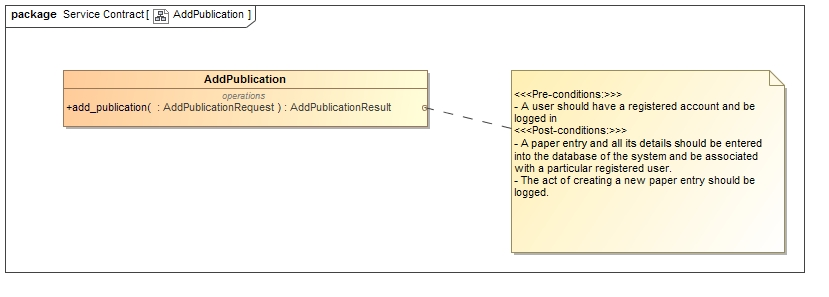
\includegraphics[width=\linewidth]{../Diagrams/AddPublication.jpg}
							\caption{Service Contract - Add Publication}
						\end{figure}
					\end{itemize}
					
					\item \textbf{Add/Remove Authors from a Paper:} \hfill \textit{Priority: Critical}
					\begin{itemize}
						\item A user should be able to add and remove authors from a paper which they have created or are a co-author of.
						\item \textbf{Pre-conditions:}
						\begin{itemize}
							\item The user must be logged in.
							\item The user must be the author or a co-author of the paper.
						\end{itemize}
						\item \textbf{Post-conditions:}
						\begin{itemize}
							\item There should be an ordered list of unlimited size associated with the paper consisting of the details of the author and co-authors stored in the database.
							\item The action should be logged.
						\end{itemize}
						\item \textbf{Request and Results Data Structures:}
					\end{itemize}
					
					\item \textbf{Create New Author:} \hfill \textit{Priority: Critical}
					\begin{itemize}
						\item A user should have the option to add the details of a new author into the system if the author does not already exist within the system.
						\item \textbf{Pre-conditions:}
						\begin{itemize}
							\item The user must be logged in.
							\item The author must not already exist. 
						\end{itemize}
						\item \textbf{Post-conditions:}
						\begin{itemize}
							\item The author and his/her associated details have been added to the system's database.
							\item The action should be logged.
						\end{itemize}
						\item \textbf{Request and Results Data Structures:}
					\end{itemize}
					
					\item \textbf{Edit Own Paper Progress:} \hfill \textit{Priority: Important}
					\begin{itemize}
						\item A user should have the ability to indicate using a percentage how far they are currently in terms of progress on their paper.
						\item \textbf{Pre-conditions:}
						\begin{itemize}
							\item A user should be logged in.
							\item The logged in user must be an author or co-author of the paper.
							\item The paper must not have been terminated.
						\end{itemize}
						\item \textbf{Post-conditions:}
						\begin{itemize}
							\item The field indicating progress within the database must have been updated.
							\item The change in progress should be depicted visually to the user.
							\item The action should be logged.
						\end{itemize}
						\item \textbf{Request and Results Data Structures:}
					\end{itemize}
					
					\item \textbf{Log Report Progress Change:} \hfill \textit{Priority: Important}
					\begin{itemize}
						\item The change of progress of a paper should be logged.
						\item \textbf{Pre-conditions:}
						\begin{itemize}
							\item The progress of a paper must have been updated.
						\end{itemize}
						\item \textbf{Post-conditions:}
						\begin{itemize}
							\item An entry must have been created in the log with all relevant details associated with the change in progress.
						\end{itemize}
						\item \textbf{Request and Results Data Structures:}
					\end{itemize}					
					
					\item \textbf{Terminate/Resume Own Paper:} \hfill \textit{Priority: Critical}
					\begin{itemize}
						\item A user must be able to terminate (make inactive) a paper which they feel they are not going to be completing in the near future. They must also be able to resume this paper at a later stage when they want to continue work on it.
						\item \textbf{Pre-conditions:}
						\begin{itemize}
							\item A user must be logged in.
							\item The logged in user must be an author or co-author of the paper.
						\end{itemize}
						\item \textbf{Post-conditions:}
						\begin{itemize}
							\item If terminating:
							\begin{itemize}
								\item The paper has been marked as terminated within the database.
								\item The action of terminating the paper must have been logged.
								\item The paper must no longer be able to be edited by the user.
							\end{itemize}
							\item If resuming:
							\begin{itemize}
								\item The paper has been unmarked as terminated within the database.
								\item The action of resuming the paper must have been logged.
								\item The paper must be available to edit.
							\end{itemize}
						\end{itemize}
						\item \textbf{Request and Results Data Structures:}
					\end{itemize}
					
					\item \textbf{Log Termination/Resuming of Paper:} \hfill \textit{Priority: Critical}
					\begin{itemize}
						\item The termination or resuming of a paper should be logged.
						\item \textbf{Pre-conditions:}
						\begin{itemize}
							\item A paper must have been terminated or resumed.
						\end{itemize}
						\item \textbf{Post-conditions:}
						\begin{itemize}
							\item An entry must have been created in the log with all relevant details associated with the termination or resuming of a paper.
						\end{itemize}
						\item \textbf{Request and Results Data Structures:}
					\end{itemize}
					
					\item \textbf{Add/Remove Conference/Journal to Paper:} \hfill \textit{Priority: Critical}
					\begin{itemize}
						\item Whilst creating or editing a paper a user should be able to associate a particular conference or journal with their paper as well as be able to remove an already associated conference or journal whilst editing a paper.
						\item \textbf{Pre-conditions:}
						\begin{itemize}
							\item The user must be logged in.
							\item The user must be an author or co-author of the paper in question.
						\end{itemize}
						\item \textbf{Post-conditions:}
						\begin{itemize}
							\item The paper should be associated with a particular conference or journal or the paper should have had its association removed.
							\item The action should be logged.
						\end{itemize}
						\item \textbf{Request and Results Data Structures:}
					\end{itemize}					
					
					\item \textbf{Log Additions and Removals:} \hfill \textit{Priority: Critical}
					\begin{itemize}
						\item The adding and removing of authors as well as conferences/journals associated with a paper should be logged.
						\item \textbf{Pre-conditions:}
						\begin{itemize}
							\item An addition or removal of an author or conference/journal must have occurred.
						\end{itemize}
						\item \textbf{Post-conditions:}
						\begin{itemize}
							\item An entry must have been created in the log with all relevant details associated with the addition or removal.
						\end{itemize}
						\item \textbf{Request and Results Data Structures:}
					\end{itemize}					
					
					\item \textbf{Create New Conference/Journal:} \hfill \textit{Priority: Critical}
					\begin{itemize}
						\item A user must be able to fill in the details of a particular conference or journal if it does not already exist within the system.
						\item \textbf{Pre-conditions:}
						\begin{itemize}
							\item The user must be logged in.
							\item The conference or journal must not already exist.
						\end{itemize}
						\item \textbf{Post-conditions:}
						\begin{itemize}
							\item The conference or journal and all its details have been added to the system's database.
							\item The action has been logged.
						\end{itemize}
						\item \textbf{Request and Results Data Structures:}
					\end{itemize}
					
					\item \textbf{Commit Changes to Database:} \hfill \textit{Priority: Critical}
					\begin{itemize}
						\item All changes to any parts of the system made by a user should be committed to the database of the system.
						\item \textbf{Pre-conditions:}
						\begin{itemize}
							\item The user must be logged in.
							\item They must have the relevant authorisation to create the changes they are making.
						\end{itemize}
						\item \textbf{Post-conditions:}
						\begin{itemize}
							\item The changes made by the user must be reflected within the database of the system and must have overwritten any old data that was present prior to the change.
						\end{itemize}
						\item \textbf{Request and Results Data Structures:}
					\end{itemize}										
				\end{itemize}
				\textbf{Head of Research:}
				
				\begin{itemize}
					\item \textbf{Search All Papers Within Own Research Group} \hfill \textit{Priority: Critical}
					\begin{itemize}
						\item The head of a research group should have access to all the papers associated with their particular research group.
						\item \textbf{Pre-conditions:}
						\begin{itemize}
							\item The user must be logged in.
							\item The user must be the head of the particular research group they would like to observe.
						\end{itemize}
						\item \textbf{Post-conditions:}
						\begin{itemize}
							\item The user should be able to view all metadata associated with the papers of their research group.
							\item The action should be logged.
						\end{itemize}
						\item \textbf{Request and Results Data Structures:}
					\end{itemize}
				\end{itemize}
				\textbf{Admin:}
				
				\begin{itemize}
					\item \textbf{Search All Papers on System} \hfill \textit{Priority: Critical}
					\begin{itemize}
						\item An admin user should be able to view all papers and their metadata on the system.
						\item \textbf{Pre-conditions:}
						\begin{itemize}
							\item The user must be logged in.
							\item The user must have the privilege rights assigned to an admin.
						\end{itemize}
						\item \textbf{Post-conditions:}
						\begin{itemize}
							\item The user should be able to view all metadata associated with all the papers stored on the system.
							\item The action should be logged.
						\end{itemize}
						\item \textbf{Request and Results Data Structures:}
					\end{itemize}
					
					\item \textbf{Purge Paper From the System} \hfill \textit{Priority: Important}
					\begin{itemize}
						\item An admin user should be able to completely remove a paper from the system if they find the need to do so.
						\item \textbf{Pre-conditions:}
						\begin{itemize}
							\item The user must be logged in.
							\item The user must have the privilege rights assigned to an admin.
						\end{itemize}
						\item \textbf{Post-conditions:}
						\begin{itemize}
							\item The paper and all of its metadata should be permanently removed from the system.
							\item The action should be logged.
						\end{itemize}
						\item \textbf{Request and Results Data Structures:}
					\end{itemize}
					
					\item \textbf{Log Paper Purge} \hfill \textit{Priority: Important}
					\begin{itemize}
						\item The act of purging a paper from the system should be logged.
						\item \textbf{Pre-conditions:}
						\begin{itemize}
							\item A paper must have been purged from the system.
						\end{itemize}
						\item \textbf{Post-conditions:}
						\begin{itemize}
							\item An entry must have been created in the log with all relevant details associated with the addition or removal.
						\end{itemize}
						\item \textbf{Request and Results Data Structures:}
					\end{itemize}
				\end{itemize}
			\cleardoublepage
			\subsubsection{User Sub-System}\label{subsubsec:user}
				Handles all actions associated with user accounts such as login, viewing and editing profiles, as well as privileged actions such as adding/removing users to the system and adding/removing users from a research group.\\
				[3mm]
				\textbf{User:}
				\begin{itemize}
					\item \textbf{Login} \hfill \textit{Priority: Critical}
					\begin{itemize}
						\item A registered user of the system must be able to login to the system using their private credentials.
						\item \textbf{Pre-conditions:}
						\begin{itemize}
							\item The user must not be logged in.
							\item The identifying field used (email address) must match one of an active, registered user of the system.
							\item The password entered must match the password associated with the identifying field within the system.
						\end{itemize}
						\item \textbf{Post-conditions:}
						\begin{itemize}
							\item The system must begin a session for the user.
							\item The user must gain access to the system according to the set of privileges associated with their account.		
							\item The action should be logged.
						\end{itemize}
						\item \textbf{Request and Results Data Structures:}
						\begin{figure}[H]
							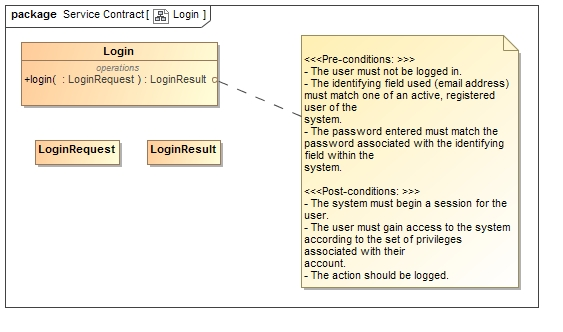
\includegraphics[width=\linewidth]{../Diagrams/ServiceContracts/Login.jpg}
							\caption{Service Contract - Login}
						\end{figure}
					\end{itemize}
					
					\cleardoublepage
					\item \textbf{Authenticate User} \hfill \textit{Priority: Critical}
					\begin{itemize}
						\item The details entered by a person attempting to login must be authenticated before they are allowed into the system.
						\item \textbf{Pre-conditions:}
						\begin{itemize}
							\item A person should have entered the requested details associated with their particular account.
						\end{itemize}
						\item \textbf{Post-conditions:}
						\begin{itemize}
							\item If the credentials were incorrect a notification must be displayed, as well as an option to reset passwords.
							\item If the credentials were correct:
							\begin{itemize}
								\item The system must begin a session for the user.
								\item The user must gain access to the system according to the set of privileges associated with their account.
								\item The user must be logged in.
							\end{itemize}													
							\item In both cases the action should be logged.
						\end{itemize}
						\item \textbf{Request and Results Data Structures:}
						\begin{figure}[H]
							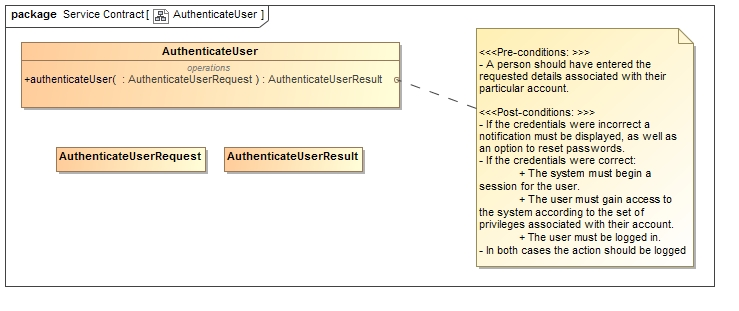
\includegraphics[width=\linewidth]{../Diagrams/ServiceContracts/AuthenticateUser.jpg}
							\caption{Service Contract - Authenticate User}
						\end{figure}
					\end{itemize}
					
					\cleardoublepage
					\item \textbf{Log Authentication Response} \hfill \textit{Priority: Critical}
					\begin{itemize}
						\item The result of a login attempt should be logged for security reasons.
						\item \textbf{Pre-conditions:}
						\begin{itemize}
							\item A login attempt needs to be made.
						\end{itemize}
						\item \textbf{Post-conditions:}
						\begin{itemize}
							\item An entry in the log needs to be made with all relevant details associated with the login attempt.
						\end{itemize}
						\item \textbf{Request and Results Data Structures:}
						\begin{figure}[H]
							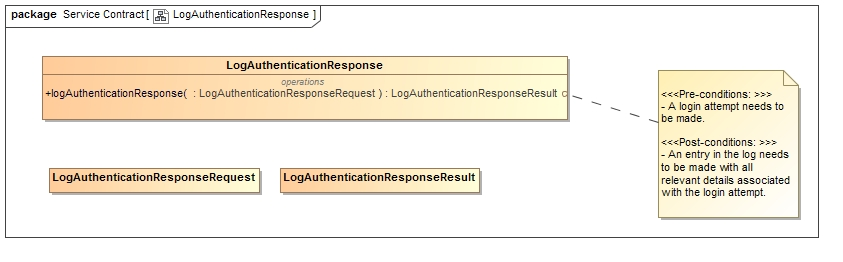
\includegraphics[width=\linewidth]{../Diagrams/ServiceContracts/LogAuthenticationResponse.jpg}
							\caption{Service Contract - Log Authentication Response}
						\end{figure}
					\end{itemize}
					
					\cleardoublepage
					\item \textbf{Logout} \hfill \textit{Priority: Critical}
					\begin{itemize}
						\item A user must be able to end their session and log out of the system.
						\item \textbf{Pre-conditions:}
						\begin{itemize}
							\item A user must be logged in.
						\end{itemize}
						\item \textbf{Post-conditions:}
						\begin{itemize}
							\item The user's session must be ended and the user must no longer be logged in.
						\end{itemize}
						\item \textbf{Request and Results Data Structures:}
						\begin{figure}[H]
							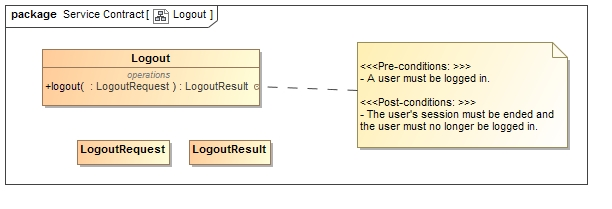
\includegraphics[width=\linewidth]{../Diagrams/ServiceContracts/Logout.jpg}
							\caption{Service Contract - Logout}
						\end{figure}
					\end{itemize}
					
					\cleardoublepage
					\item \textbf{View Own User Profile} \hfill \textit{Priority: Critical}
					\begin{itemize}
						\item A logged in user should be able to see their own profile and all details associated with it. The user should also be able to view all papers associated with their account.
						\item \textbf{Pre-conditions:}
						\begin{itemize}
							\item The user must be logged in.
							\item The user's profile being viewed must be the same as the logged in user.
						\end{itemize}
						\item \textbf{Post-conditions:}
						\begin{itemize}
							\item The information associated with the user's account should be displayed to them.
							\item The action should be logged.
						\end{itemize}
						\item \textbf{Request and Results Data Structures:}
						\begin{figure}[H]
							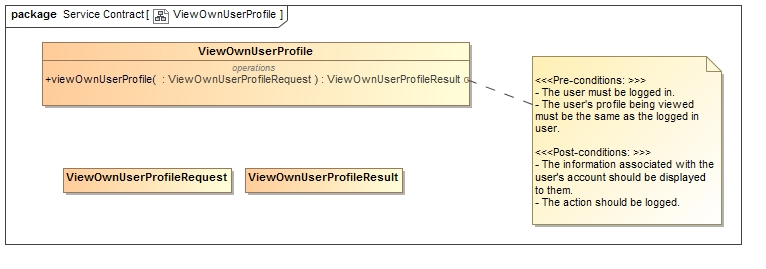
\includegraphics[width=\linewidth]{../Diagrams/ServiceContracts/ViewOwnUserProfile.jpg}
							\caption{Service Contract - View Own User Profile}
						\end{figure}
					\end{itemize}
					
					\cleardoublepage
					\item \textbf{Edit Own User Profile} \hfill \textit{Priority: Critical}
					\begin{itemize}
						\item A logged in user should be able to edit all details associated with their user account.
						\item \textbf{Pre-conditions:}
						\begin{itemize}
							\item The user must be logged in.
							\item The user profile being edited must belong to the user editing it.
						\end{itemize}
						\item \textbf{Post-conditions:}
						\begin{itemize}
							\item The updated information associated with the user's account should be stored in the system.
							\item The action should be logged.
						\end{itemize}
						\item \textbf{Request and Results Data Structures:}
						\begin{figure}[H]
							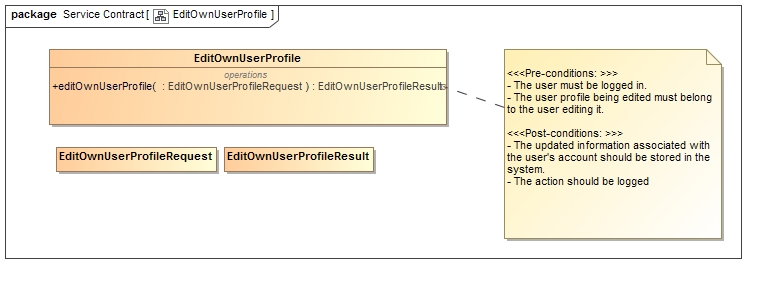
\includegraphics[width=\linewidth]{../Diagrams/ServiceContracts/EditOwnUserProfile.jpg}
							\caption{Service Contract - Edit Own User Profile}
						\end{figure}
					\end{itemize}							
				\end{itemize}
				\cleardoublepage
				\textbf{Head of Research:}
				
				\begin{itemize}
					\item \textbf{Add/Remove Users from Own Research Group} \hfill \textit{Priority: Critical}
					\begin{itemize}
						\item The head of a research group should be able to manage the users associated with that group.
						\item \textbf{Pre-conditions:}
						\begin{itemize}
							\item The user must be logged in.
							\item The user must have the privileges associated with a Head of Research.
							\item The user must be the Head of Research of the particular group which they are wanting to manage.
						\end{itemize}
						\item \textbf{Post-conditions:}
						\begin{itemize}
							\item The user must have been able to add other registered users into their research group.
							\item The user must have been able to remove other registered users from their research group.
							\item The action should be logged.
						\end{itemize}
						\item \textbf{Request and Results Data Structures:}
						\begin{figure}[H]
							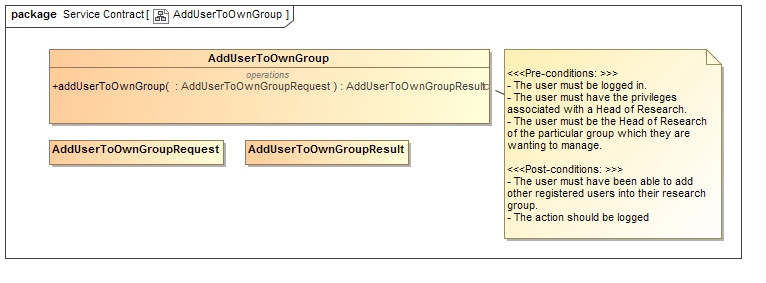
\includegraphics[width=\linewidth]{../Diagrams/ServiceContracts/AddUserToOwnGroup.jpg}
							\caption{Service Contract - Add User to Own Group}
						\end{figure}
						\begin{figure}[H]
							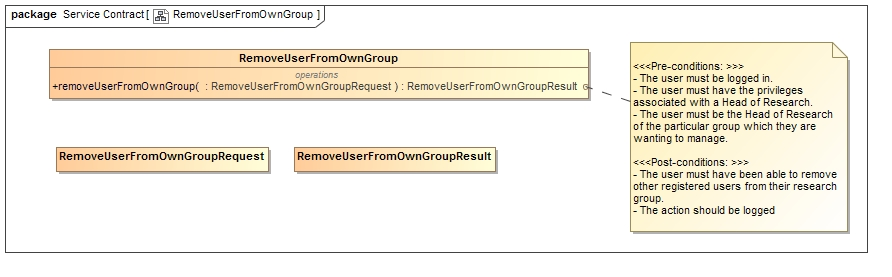
\includegraphics[width=\linewidth]{../Diagrams/ServiceContracts/RemoveUserFromOwnGroup.jpg}
							\caption{Service Contract - Remove User from Own Group}
						\end{figure}
					\end{itemize}
					
					\cleardoublepage
					\item \textbf{Search/View All Users in Own Research Group} \hfill \textit{Priority: Critical}
					\begin{itemize}
						\item The head of a research group should be able to search all of the users within their research group. They should also be able to access the profiles and information associated with the users within their research group. In particular the head of a research group should be able to view all paper entries associated with each user.
						\item \textbf{Pre-conditions:}
						\begin{itemize}
							\item The user must be logged in.
							\item The user must be the Head of Research of the particular group which they are wanting to search/view.
						\end{itemize}
						\item \textbf{Post-conditions:}
						\begin{itemize}
							\item The user must have been able to view all of the users associated with their research group.
							\item The head of the research group can access and view all profile information (including paper entries) for each of the users associated with their research group.
							\item The action should be logged.
						\end{itemize}
						\item \textbf{Request and Results Data Structures:}
						\begin{figure}[H]
							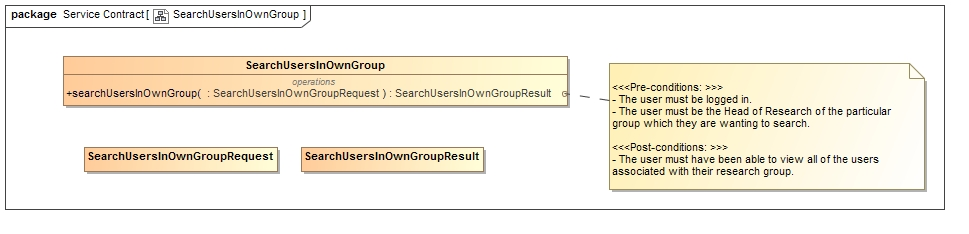
\includegraphics[width=\linewidth]{../Diagrams/ServiceContracts/SearchUsersInOwnGroup.jpg}
							\caption{Service Contract - Search Users in Own Group}
						\end{figure}
						\begin{figure}[H]
							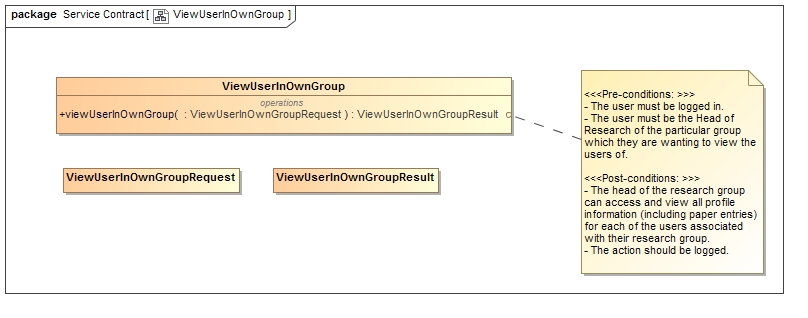
\includegraphics[width=\linewidth]{../Diagrams/ServiceContracts/ViewUserInOwnGroup.jpg}
							\caption{Service Contract - View User in Own Group}
						\end{figure}
					\end{itemize}
				\end{itemize}
				
				\cleardoublepage
				\textbf{Admin:}
				
				\begin{itemize}
					\item \textbf{Add New User to System} \hfill \textit{Priority: Critical}
					\begin{itemize}
						\item Admin users should have the ability to add new users into the system.
						\item \textbf{Pre-conditions:}
						\begin{itemize}
							\item The user must be logged in.
							\item The user must have the privileges associated with an admin account.
						\end{itemize}
						\item \textbf{Post-conditions:}
						\begin{itemize}
							\item A new user with all their metadata as well as privileges should be added into the system.
							\item The action should be logged.
						\end{itemize}
						\item \textbf{Request and Results Data Structures:}
						\begin{figure}[H]
							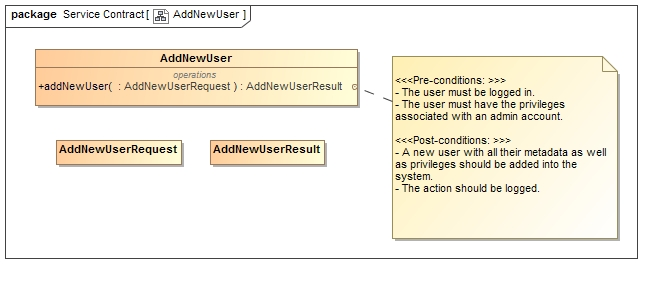
\includegraphics[width=\linewidth]{../Diagrams/ServiceContracts/AddNewUser.jpg}
							\caption{Service Contract - Add New User}
						\end{figure}
					\end{itemize}
					
					\cleardoublepage
					\item \textbf{Search/View All Users in Any Research Group} \hfill \textit{Priority: Critical}
					\begin{itemize}
						\item Admin users should be able to search through all of the users within the system as well as view their profiles and all associated data and papers.
						\item \textbf{Pre-conditions:}
						\begin{itemize}
							\item The user must be logged in.
							\item The user must have the privileges associated with an admin account.
						\end{itemize}
						\item \textbf{Post-conditions:}
						\begin{itemize}
							\item The admin user should have been able to search and locate particular registered users on the system.
							\item All information, paper entries and their metadata should be available for viewing to the admin user. Upon selecting a particular user all information associated with that user is displayed.
							\item This action should be logged.
						\end{itemize}
						\item \textbf{Request and Results Data Structures:}
						\begin{figure}[H]
							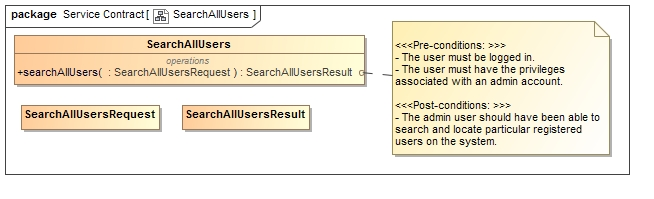
\includegraphics[width=\linewidth]{../Diagrams/ServiceContracts/SearchAllUsers.jpg}
							\caption{Service Contract - Search All Users}
						\end{figure}
						\begin{figure}[H]
							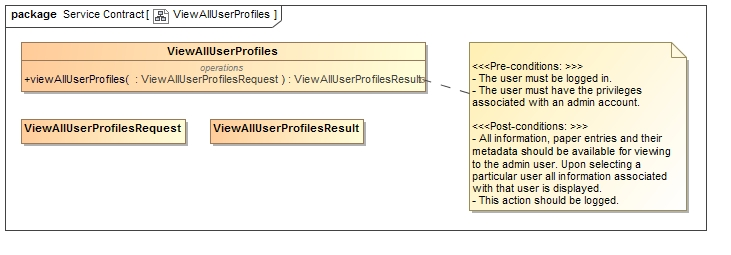
\includegraphics[width=\linewidth]{../Diagrams/ServiceContracts/ViewAllUserProfiles.jpg}
							\caption{Service Contract - View All User Profiles}
						\end{figure}
					\end{itemize}
					
					\cleardoublepage
					\item \textbf{Purge User from System} \hfill \textit{Priority: Nice-to-Have}
					\begin{itemize}
						\item An admin user must be able to permanently remove a user and all of their associated information from the system.
						\item \textbf{Pre-conditions:}
						\begin{itemize}
							\item The user must be logged in.
							\item The user must have the privileges associated with an admin account.
							\item The user must confirm they want to continue with the action before the system executes the command.
						\end{itemize}
						\item \textbf{Post-conditions:}
						\begin{itemize}
							\item The user and all of their associated information should be removed from the system.
							\item The action should be logged.
						\end{itemize}
						\item \textbf{Request and Results Data Structures:}
						\begin{figure}[H]
							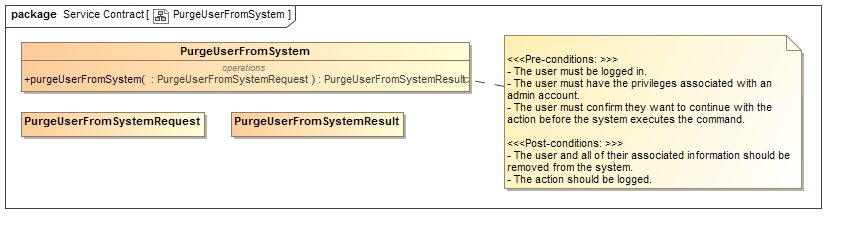
\includegraphics[width=\linewidth]{../Diagrams/ServiceContracts/PurgeUserFromSystem.jpg}
							\caption{Service Contract - Purge User From System}
						\end{figure}
					\end{itemize}
					
					\cleardoublepage
					\item \textbf{Set User as Active/Inactive} \hfill \textit{Priority: Important}
					\begin{itemize}
						\item An admin user should be able to set the status of a user to active or inactive, allowing the user to login or preventing them from continuing to interact with the system.
						\item \textbf{Pre-conditions:}
						\begin{itemize}
							\item The user must be logged in.
							\item The user must have the privileges associated with an admin account.
						\end{itemize}
						\item \textbf{Post-conditions:}
						\begin{itemize}
							\item The selected user should have been marked as active/inactive, active allowing the user to login and use the system, inactive preventing them from login in to the system and making changes.
							\item The action should be logged.
						\end{itemize}
						\item \textbf{Request and Results Data Structures:}
						\begin{figure}[H]
							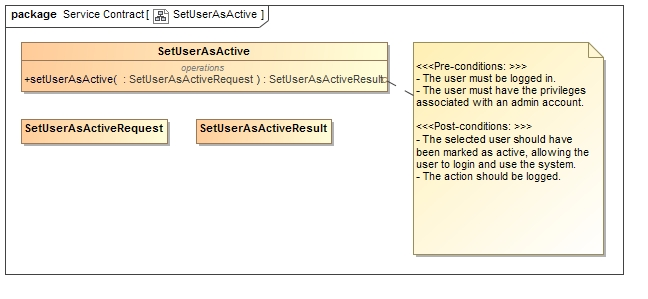
\includegraphics[width=\linewidth]{../Diagrams/ServiceContracts/SetUserAsActive.jpg}
							\caption{Service Contract - Set User as Active}
						\end{figure}
						\begin{figure}[H]
							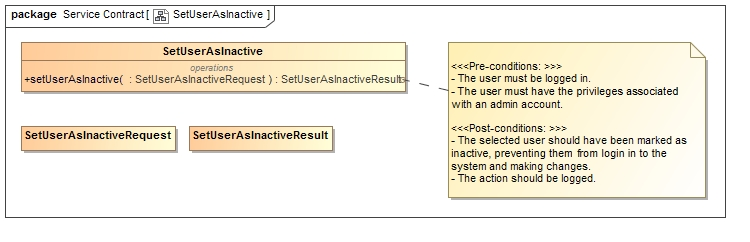
\includegraphics[width=\linewidth]{../Diagrams/ServiceContracts/SetUserAsInactive.jpg}
							\caption{Service Contract - Set User as Inactive}
						\end{figure}
					\end{itemize}
					
					\cleardoublepage
					\item \textbf{Add/Remove Users From Any Research Group} \hfill \textit{Priority: Critical}
					\begin{itemize}
						\item An admin user should be able to add or remove a user from any of the research groups within the system.
						\item \textbf{Pre-conditions:}
						\begin{itemize}
							\item The user must be logged in.
							\item The user must have the privileges associated with an admin account.
						\end{itemize}
						\item \textbf{Post-conditions:}
						\begin{itemize}
							\item The selected user should be associated with the specified research group in the case of adding and should be removed and no longer associated with a research group in the case of removing.
							\item The action should be logged.
						\end{itemize}
						\item \textbf{Request and Results Data Structures:}
						\begin{figure}[H]
							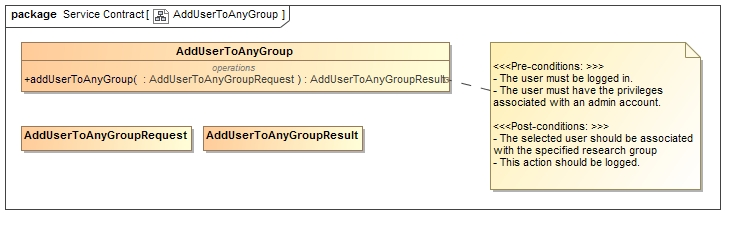
\includegraphics[width=\linewidth]{../Diagrams/ServiceContracts/AddUserToAnyGroup.jpg}
							\caption{Service Contract - Add User to Any Group}
						\end{figure}
						\begin{figure}[H]
							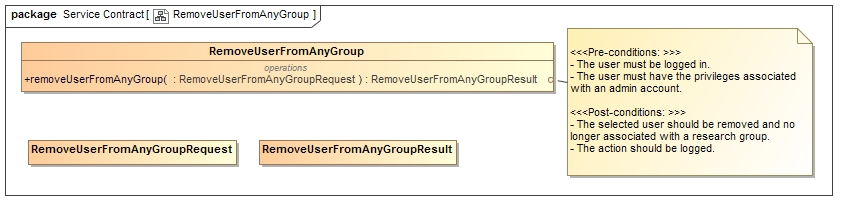
\includegraphics[width=\linewidth]{../Diagrams/ServiceContracts/RemoveUserFromAnyGroup.jpg}
							\caption{Service Contract - Remove User from Any Group}
						\end{figure}
					\end{itemize}
				\end{itemize}
				
				\cleardoublepage
			\subsubsection{Notification Sub-System}\label{subsubsec:notification}
				Handles the adding and editing of notifications within the system, as well the process of creating and sending notifications to relevant users of the system.\\
				[3mm]
				\textbf{User:}
				\begin{itemize}
					\item \textbf{Add/Update Paper Deadline} \hfill \textit{Priority: Important}
					\begin{itemize}
						\item Upon creating a paper entry a user must be able to set the deadline for when the paper needs to be published by. As well as being able to edit the deadline associated with their papers.
						\item \textbf{Pre-conditions:}
						\begin{itemize}
							\item The user must be logged in.
							\item The user must be the author or a co-author of the paper which they would like to set the deadline for.
							\item The paper must not have been terminated.
						\end{itemize}
						\item \textbf{Post-conditions:}
						\begin{itemize}
							\item A deadline will have been set and stored in the system. It will be associated with the particular paper on which it was set in the case of adding.
							\item In the case of updating the change in the deadline should reflect within the system and overwrite the previous deadline.
							\item An update notification should be sent to authors of the paper indicating that the deadline was changed.
							\item The action should be logged.
						\end{itemize}
						\item \textbf{Request and Results Data Structures:}
						\begin{figure}[H]
							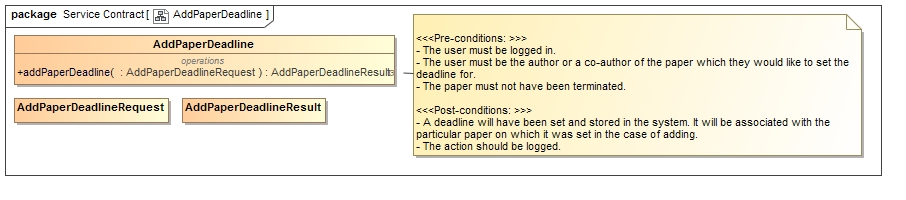
\includegraphics[width=\linewidth]{../Diagrams/ServiceContracts/AddPaperDeadline.jpg}
							\caption{Service Contract - Add Paper Deadline}
						\end{figure}
						\begin{figure}[H]
							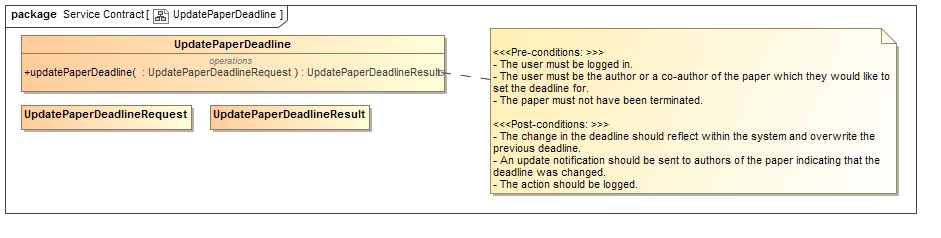
\includegraphics[width=\linewidth]{../Diagrams/ServiceContracts/UpdatePaperDeadline.jpg}
							\caption{Service Contract - Update Paper Deadline}
						\end{figure}
					\end{itemize}	
					
					\item \textbf{Send Deadline Update Notification} \hfill \textit{Priority: Important}
					\begin{itemize}
						\item The system must be able to notify an author as well as co-authors of a paper when the deadline for a paper is updated.
						\item \textbf{Pre-conditions:}
						\begin{itemize}
							\item The user must be logged in.
							\item A new deadline must have been set for a paper.
							\item The deadline must not have passed already.
							\item The authors being notified must be associated with the paper the deadline has been updated on.
						\end{itemize}
						\item \textbf{Post-conditions:}
						\begin{itemize}
							\item Authors of a particular paper are notified via the use of email as to what the updated deadline for the paper is.
							\item The action should be logged.
						\end{itemize}
						\item \textbf{Request and Results Data Structures:}
					\end{itemize}						
				\end{itemize}
				\textbf{\large{Date and Time:}}
				\begin{itemize}
					\item \textbf{Send Deadline Notification} \hfill \textit{Priority: Important}
					\begin{itemize}
						\item The system must be able to notify an author as well as co-authors of a paper of the deadline for the paper.
						\item \textbf{Pre-conditions:}
						\begin{itemize}
							\item A deadline must have been set for a paper.
							\item The deadline must not have passed already.
							\item The authors being notified must be associated with the paper the deadline has been set on.
						\end{itemize}
						\item \textbf{Post-conditions:}
						\begin{itemize}
							\item Authors of a particular paper are notified via the use of email as to what the deadline for the paper is.
							\item The action should be logged.
						\end{itemize}
						\item \textbf{Request and Results Data Structures:}
						\begin{figure}[H]
							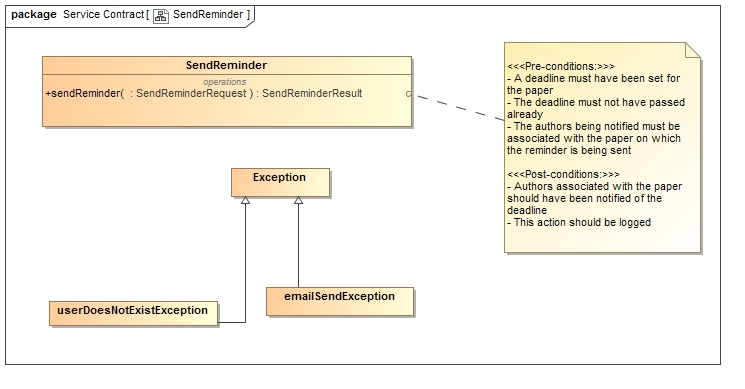
\includegraphics[width=\linewidth]{../Diagrams/SendReminder.jpg}
							\caption{Service Contract - Send Reminder}
						\end{figure}
					\end{itemize}
				\end{itemize}
			\subsubsection{Reporting Sub-System}\label{subsubsec:report}
				Handles the generation of reports with regards to all relevant information contained by the system.\\
				[3mm]
				\textbf{Head of Research:}
				\begin{itemize}
					\item \textbf{Generate Report for Research Group} \hfill \textit{Priority: Critical}
					\begin{itemize}
						\item The head of a research group should be able to generate a summarised report of all important information related to their research group in terms of the users in the group as well as their papers and all metadata associated with their papers.
						\item \textbf{Pre-conditions:}
						\begin{itemize}
							\item The user must be logged in.
							\item The user must have the privileges associated with a Head of Research.
							\item The user must be the head of the research group which they would like to generate a report on.
						\end{itemize}
						\item \textbf{Post-conditions:}
						\begin{itemize}
							\item The head of the research group should have all relevant information returned to him/her in a summarised and easily readable manner.
							\item This action should be logged.
						\end{itemize}
						\item \textbf{Request and Results Data Structures:}
					\end{itemize}
				\end{itemize}
				\textbf{Admin:}
				\begin{itemize}
					\item \textbf{Generate Report for Department} \hfill \textit{Priority: Critical}
					\begin{itemize}
						\item An admin user should be able to generate a summarised report of all important information related to their department as a whole. This includes summaries of each research group and associated papers, as well as of each individual user of the system and their associated papers.
						\item \textbf{Pre-conditions:}
						\begin{itemize}
							\item The user must be logged in.
							\item The user must have the privileges associated with an admin.
						\end{itemize}
						\item \textbf{Post-conditions:}
						\begin{itemize}
							\item The admin should have all relevant information returned to him/her in a summarised and easily readable manner.
							\item The action should be logged.
						\end{itemize}
						\item \textbf{Request and Results Data Structures:}
					\end{itemize}

					\item \textbf{Dump Database to File} \hfill \textit{Priority: Critical}
					\begin{itemize}
						\item An admin user should be able to at any point dump all of the information within the database into a file for safekeeping, such as a CSV file.
						\item \textbf{Pre-conditions:}
						\begin{itemize}
							\item The user must be logged in.
							\item The user must have the privileges associated with an admin user.
						\end{itemize}
						\item \textbf{Post-conditions:}
						\begin{itemize}
							\item All information contained in the database should be dumped into a CSV file and be made available to download by the admin user.
							\item This action should be logged.
						\end{itemize}
						\item \textbf{Request and Results Data Structures:}
					\end{itemize}
				\end{itemize}
			\subsubsection{Group-Control Sub-System}\label{subsubsec:group}
				Handles the creating and removing of research groups, as well as the allocating of heads of research groups and the editing of individual research groups associated metadata.\\
				[3mm]
				\textbf{Head of Research:}
				\begin{itemize}
					\item \textbf{Edit Research Group Information} \hfill \textit{Priority: Critical}
					\begin{itemize}
						\item A head of a research group should be able to edit the information associated with their research group.
						\item \textbf{Pre-conditions:}
						\begin{itemize}
							\item The user must be logged in.
							\item The user must have the privileges associated with a research leader.
							\item The user must be the head of the research group which they are attempting to edit the information of.
						\end{itemize}
						\item \textbf{Post-conditions:}
						\begin{itemize}
							\item The information associated with the particular research group should have been updated within the system.
							\item This action should be logged.
						\end{itemize}
						\item \textbf{Request and Results Data Structures:}
					\end{itemize}
				\end{itemize}
				\textbf{Admin:}
				\begin{itemize}
					\item \textbf{Add/Remove Research Groups} \hfill \textit{Priority: Critical}
					\begin{itemize}
						\item An admin user should be able to add or remove research groups from the system.
						\item \textbf{Pre-conditions:}
						\begin{itemize}
							\item The user must be logged in.
							\item The user must have the privileges associated with an admin user.
						\end{itemize}
						\item \textbf{Post-conditions:}
						\begin{itemize}
							\item In the case of adding a new research group which is able to have users added to or removed from should exist within the system.
							\item In the case of removing a research group the group should be removed from the system as well as all relationships related to users contained within the group.
							\item In both instances the action should be logged.
						\end{itemize}
						\item \textbf{Request and Results Data Structures:}
					\end{itemize}

					\item \textbf{Edit Any Research Groups Information} \hfill \textit{Priority: Critical}
					\begin{itemize}
						\item An admin user should be able to edit the information associated with any of the research groups within the system.
						\item \textbf{Pre-conditions:}
						\begin{itemize}
							\item The user must be logged in.
							\item The user must have the privileges associated with an admin user.
						\end{itemize}
						\item \textbf{Post-conditions:}
						\begin{itemize}
							\item The information associated with the particular research group should have been updated within the system.
							\item This action should be logged.
						\end{itemize}
						\item \textbf{Request and Results Data Structures:}
					\end{itemize}

					\item \textbf{Allocate/Change Head of Research Group} \hfill \textit{Priority: Critical}
					\begin{itemize}
						\item An admin user should be able to allocate a registered user to be the head of a particular research group, in turn allowing for this user to have more privileges within the system. An admin user should also be able to change the head of a research group.
						\item \textbf{Pre-conditions:}
						\begin{itemize}
							\item The user must be logged in.
							\item The user must have the privileges associated with an admin user.
						\end{itemize}
						\item \textbf{Post-conditions:}
						\begin{itemize}
							\item In the case of allocating the allocated user should now have the necessary rights and privileges to manage and view their allocated research group.
							\item In the case of changing the old head of a research group should have their privileges removed and the new head should be granted those privileges.
							\item This action should be logged.
						\end{itemize}
						\item \textbf{Request and Results Data Structures:}
					\end{itemize}
				\end{itemize}
				\subsubsection{Logging Sub-System}\label{subsubsec:logging}
				Handles the logging of all important interactions which take place on the system.\\
				[3mm]
				\textbf{Admin:}
				\begin{itemize}
					\item \textbf{Download and View Log Text Files} \hfill \textit{Priority: Critical}
					\begin{itemize}
						\item An admin user should be able to download a text file containing the logs of the system.
						\item \textbf{Pre-conditions:}
						\begin{itemize}
							\item The user must be logged in.
							\item The user must have the privileges associated with an admin.
						\end{itemize}
						\item \textbf{Post-conditions:}
						\begin{itemize}
							\item A file should be made available to download containing all the relevant logs which the admin requested.
						\end{itemize}
						\item \textbf{Request and Results Data Structures:}
					\end{itemize}
				\end{itemize}
				\textbf{Date and Time:}
				\begin{itemize}
					\item \textbf{Move Current Log File to Backup} \hfill \textit{Priority: Critical}
					\begin{itemize}
						\item The system should periodically backup the current log file.
						\item \textbf{Pre-conditions:}
						\begin{itemize}
							\item A certain period of time must have passed.
						\end{itemize}
						\item \textbf{Post-conditions:}
						\begin{itemize}
							\item The old log file should have been backed up.
							\item A new log file should be created.
						\end{itemize}
						\item \textbf{Request and Results Data Structures:}
					\end{itemize}
					
					\item \textbf{Create New Log File} \hfill \textit{Priority: Critical}
					\begin{itemize}
						\item After backing up the previous log file a new one should be created in order to replace the previous one.
						\item \textbf{Pre-conditions:}
						\begin{itemize}
							\item The old log file must have been backed up.
						\end{itemize}
						\item \textbf{Post-conditions:}
						\begin{itemize}
							\item A new log file should replace the older log file so that it can record any future logs.
						\end{itemize}
						\item \textbf{Request and Results Data Structures:}
					\end{itemize}
				\end{itemize}
			
		\subsection{Required Functionality}\label{subsec:requiredfunctionionality}
			%\begin{figure}[h]
			%\includegraphics[width=4in]{imagename}
			%\caption{Figure information}
			%\end
	
		\subsection{Process Specifications}\label{subsec:processspecification}
		Certain use cases require further information with regards to their function.\\ These use cases are specified further by means of process specification.
		\subsubsection{User Sub-System}
			\begin{figure}[H]
				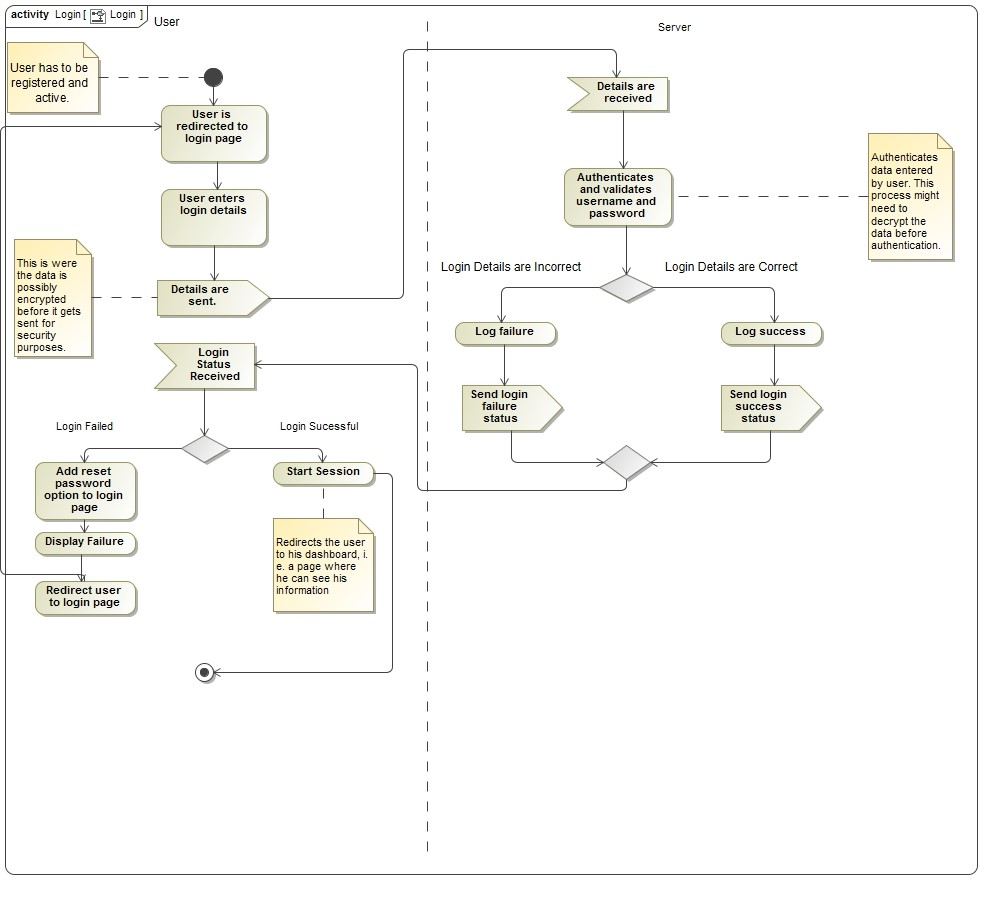
\includegraphics[width=4in, center]{../Diagrams/Process Specifications/Login.jpg}
				\caption{User - Login}
			\end{figure}
			\begin{figure}[H]
				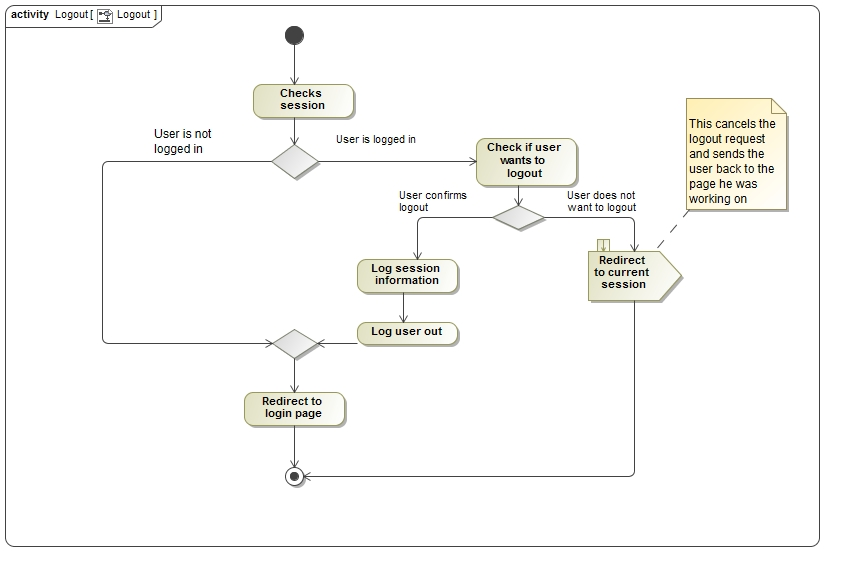
\includegraphics[width=4in, center]{../Diagrams/Process Specifications/act__Logout__Logout.jpg}
				\caption{User - Logout}
			\end{figure}
			\begin{figure}[H]
				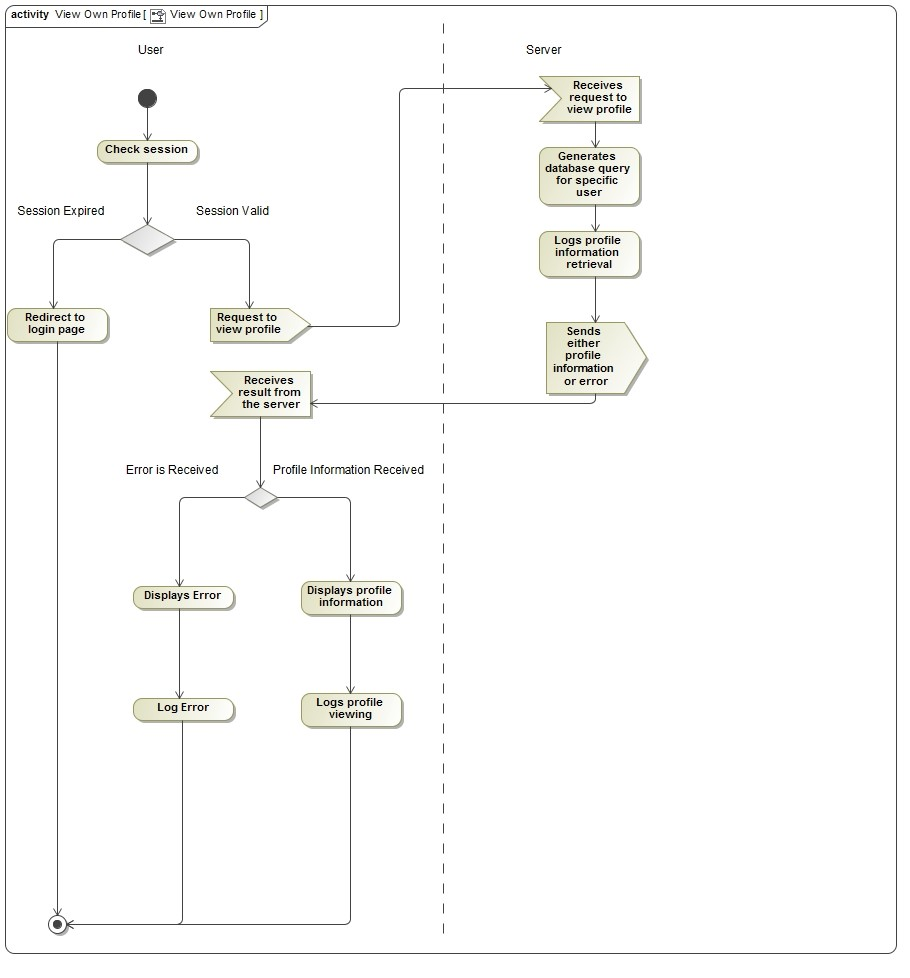
\includegraphics[width=4in, center]{../Diagrams/Process Specifications/View Own Profile.jpg}
				\caption{User - View Own Profile}
			\end{figure}
			\begin{figure}[H]
				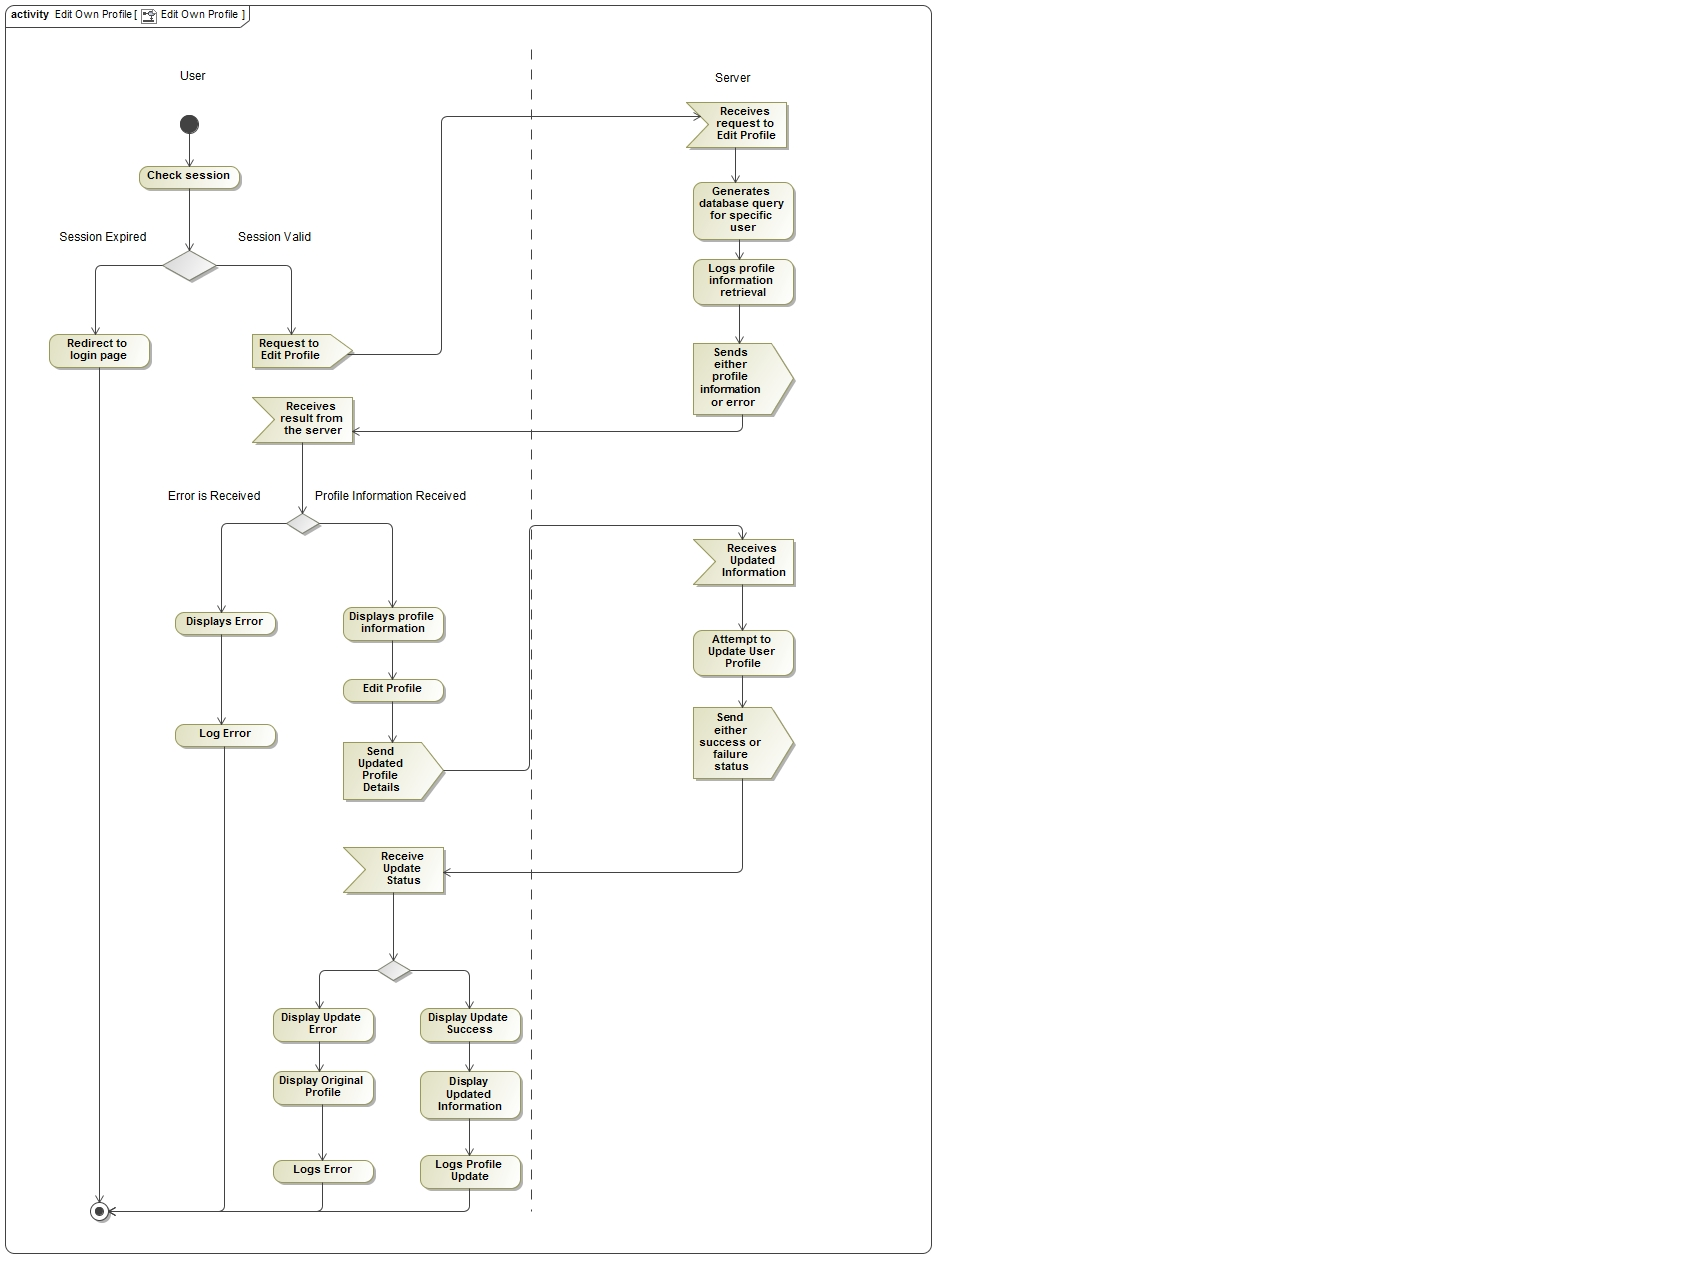
\includegraphics[width=4in, center]{../Diagrams/Process Specifications/Edit Own Profile.jpg}
				\caption{User - Edit Own Profile}
			\end{figure}
			\begin{figure}[H]
				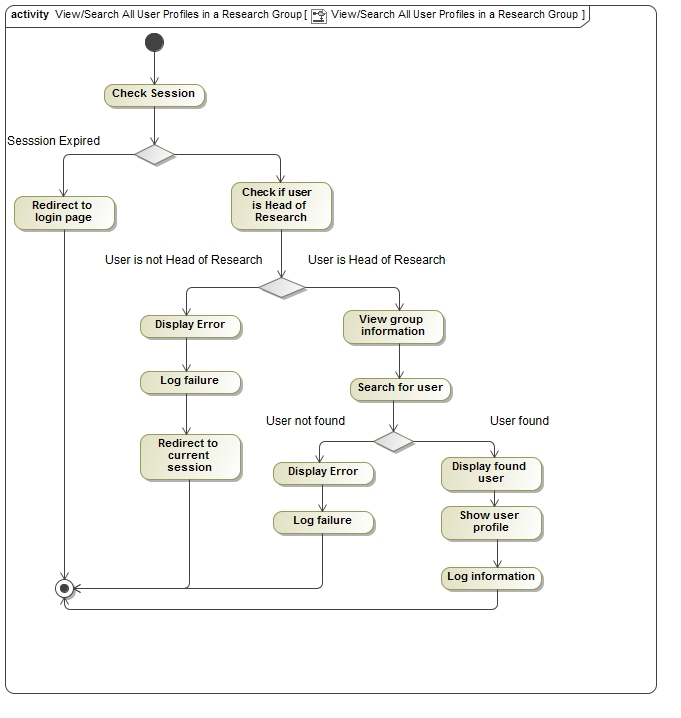
\includegraphics[width=4in, center]{../Diagrams/Process Specifications/View_Search All User Profiles in a Research Group.jpg}
				\caption{Head of Research - Search/View All Users in a Research Group}
			\end{figure}
			\begin{figure}[H]
				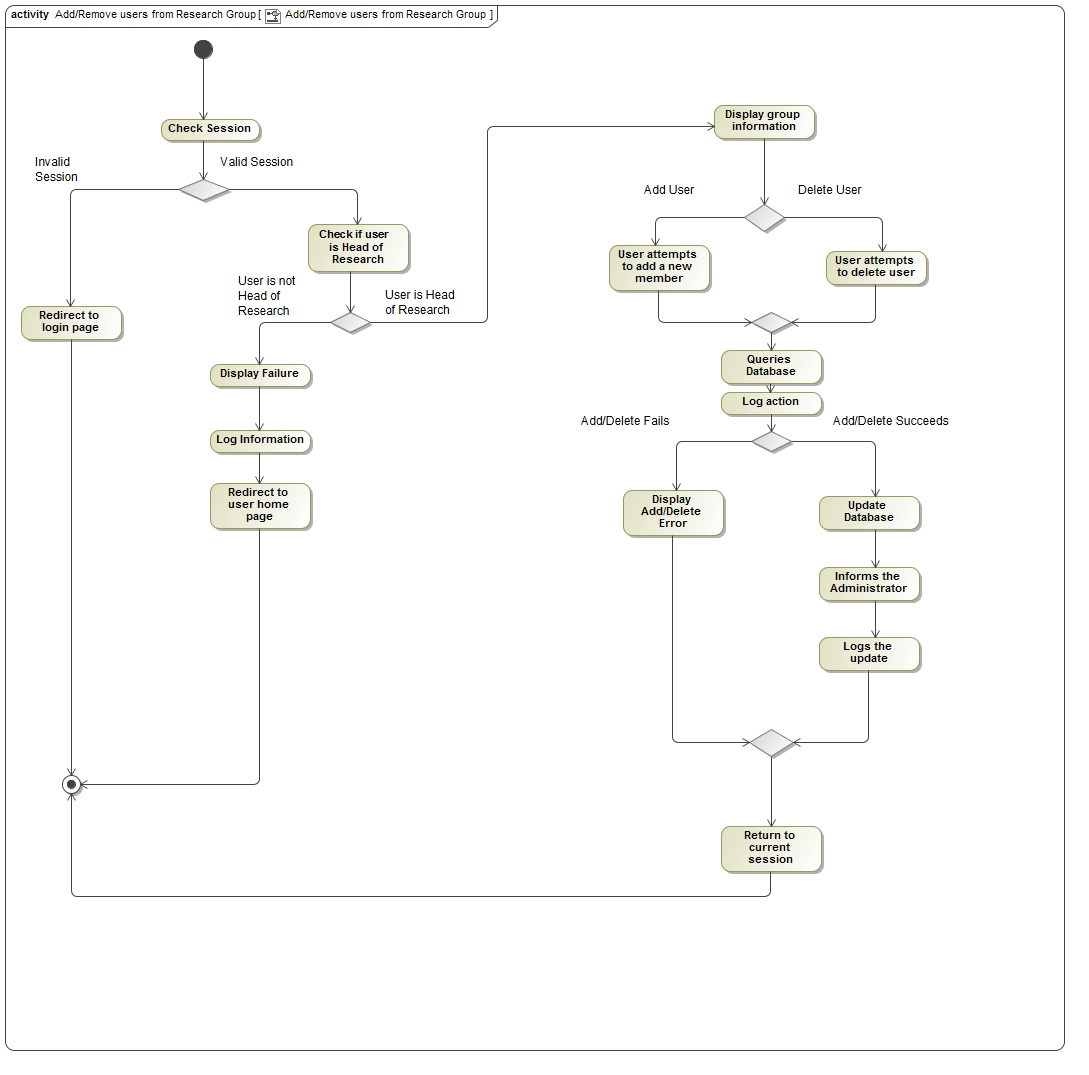
\includegraphics[width=4in, center]{../Diagrams/Process Specifications/Add_Remove Users from Research Group.jpg}
				\caption{Head of Research - Add/Remove All Users in a Research Group}
			\end{figure}
			\begin{figure}[H]
				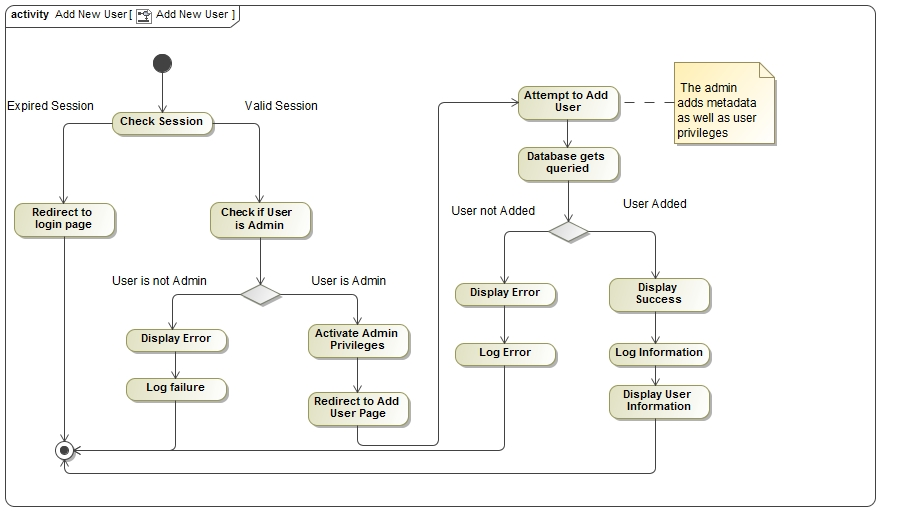
\includegraphics[width=4in, center]{../Diagrams/Process Specifications/Add New User.jpg}
				\caption{Admin - Add New User to System}
			\end{figure}
			\begin{figure}[H]
				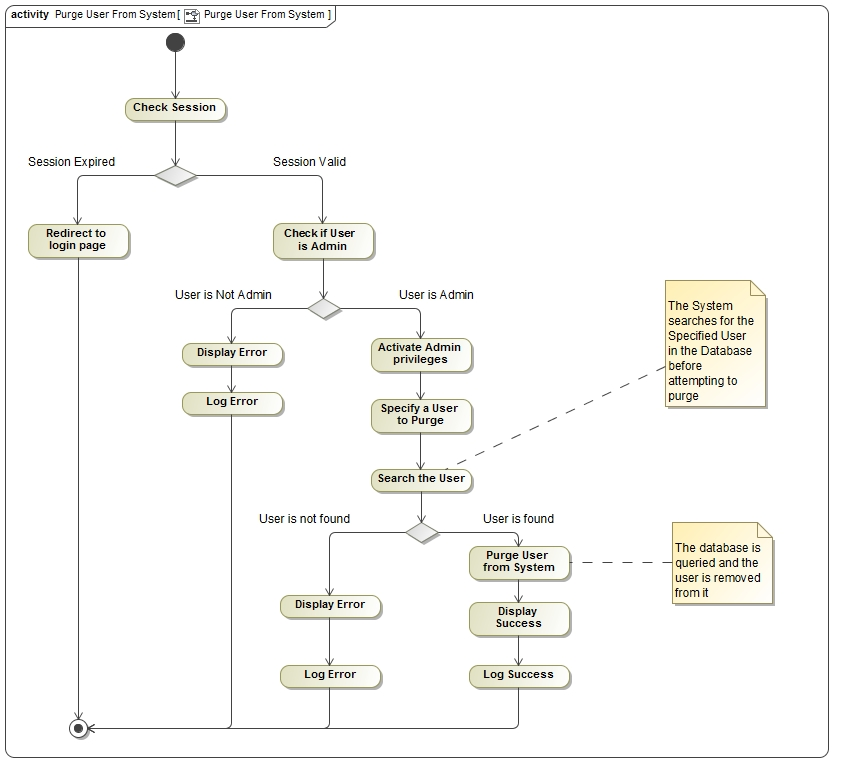
\includegraphics[width=4in, center]{../Diagrams/Process Specifications/Purge User From System.jpg}
				\caption{Admin - Purge User from System}
			\end{figure}
			\begin{figure}[H]
				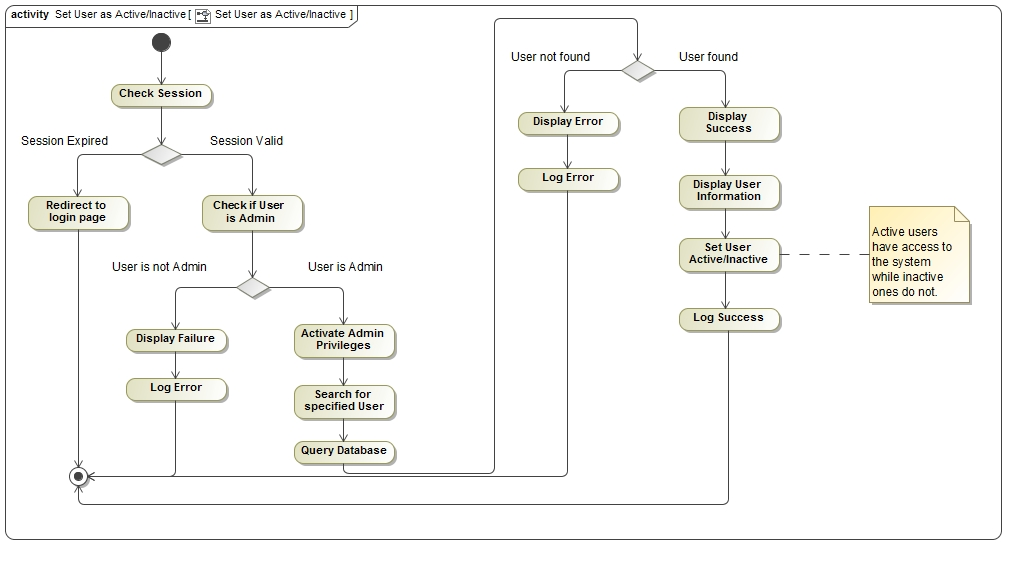
\includegraphics[width=4in, center]{../Diagrams/Process Specifications/Set User as Active_Inactive.jpg}
				\caption{Admin - Set User as Active or Inactive}
			\end{figure}
			\begin{figure}[H]
				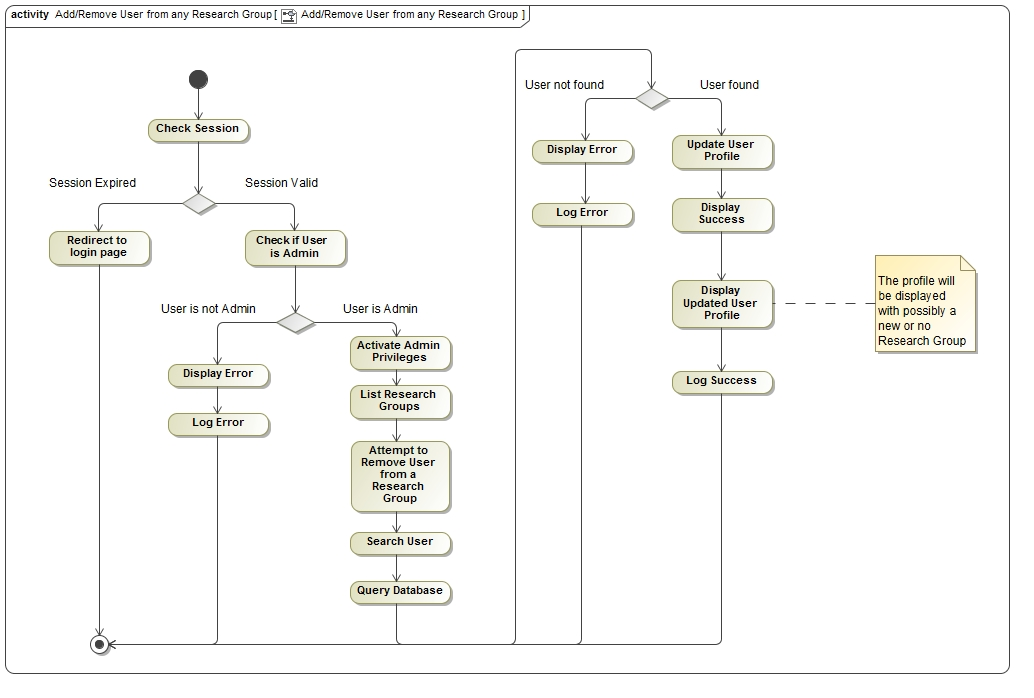
\includegraphics[width=4in, center]{../Diagrams/Process Specifications/Add_Remove User from any Research Group.jpg}
				\caption{Admin - Add/Remove Users from any Research Group}
			\end{figure}
			\begin{figure}[H]
				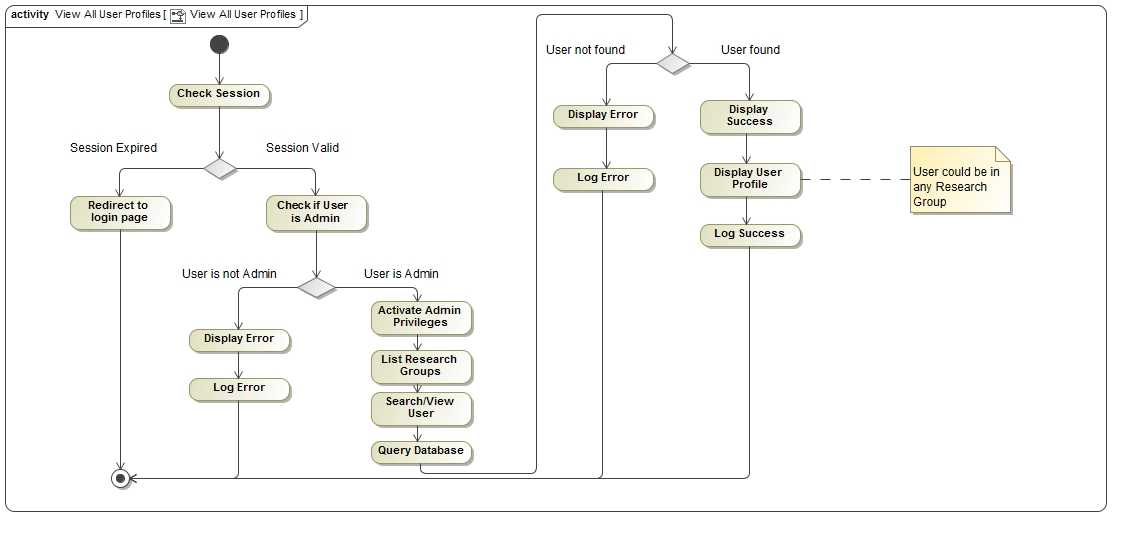
\includegraphics[width=4in, center]{../Diagrams/Process Specifications/View All User Profiles.jpg}
				\caption{Admin - Search/View All Users in any Research Group}
			\end{figure}
			
			\subsubsection{Notification Sub-System}
			\begin{figure}[H]
				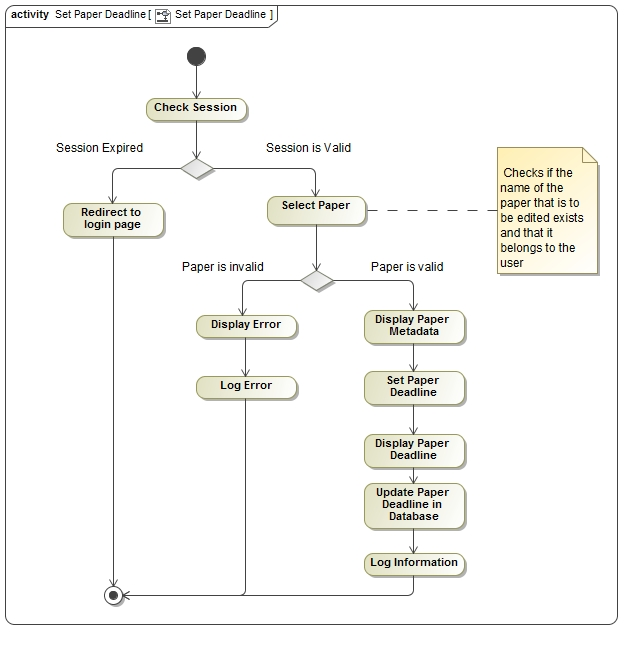
\includegraphics[width=4in, center]{../Diagrams/Process Specifications/Set Paper Deadline.jpg}
				\caption{User - Set Paper Deadline}
			\end{figure}
			\begin{figure}[H]
				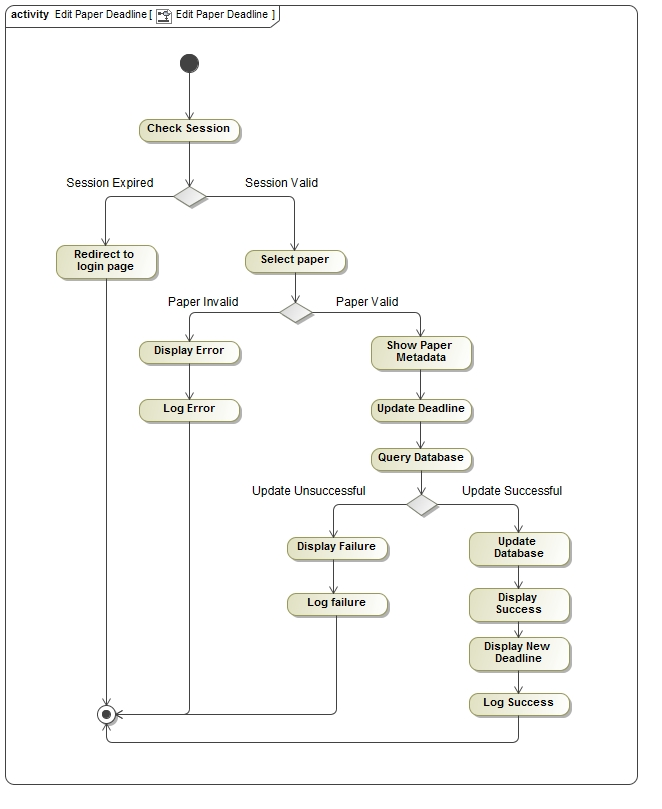
\includegraphics[width=4in, center]{../Diagrams/Process Specifications/Edit Paper Deadline.jpg}
				\caption{User - Edit Paper Deadline}
			\end{figure}
			\begin{figure}[H]
				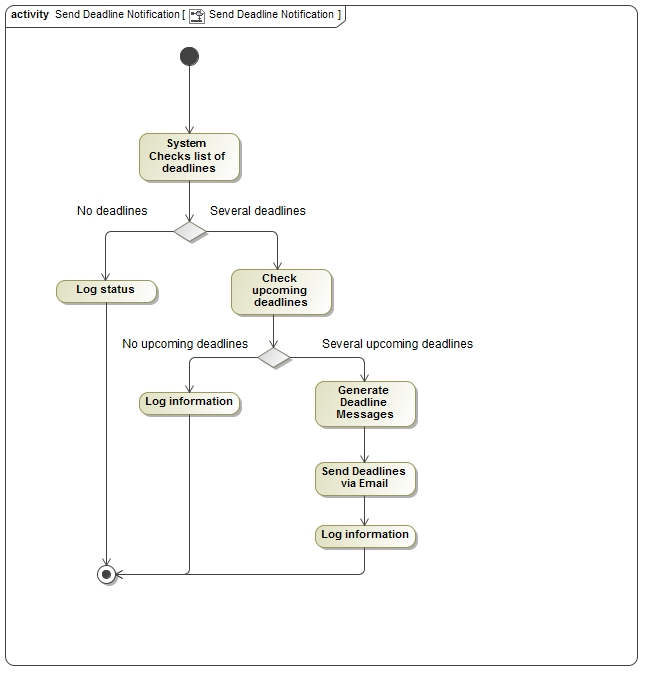
\includegraphics[width=4in, center]{../Diagrams/Process Specifications/Send Deadline Notification.jpg}
				\caption{System - Send Deadline Notification}
			\end{figure}
			\begin{figure}[H]
				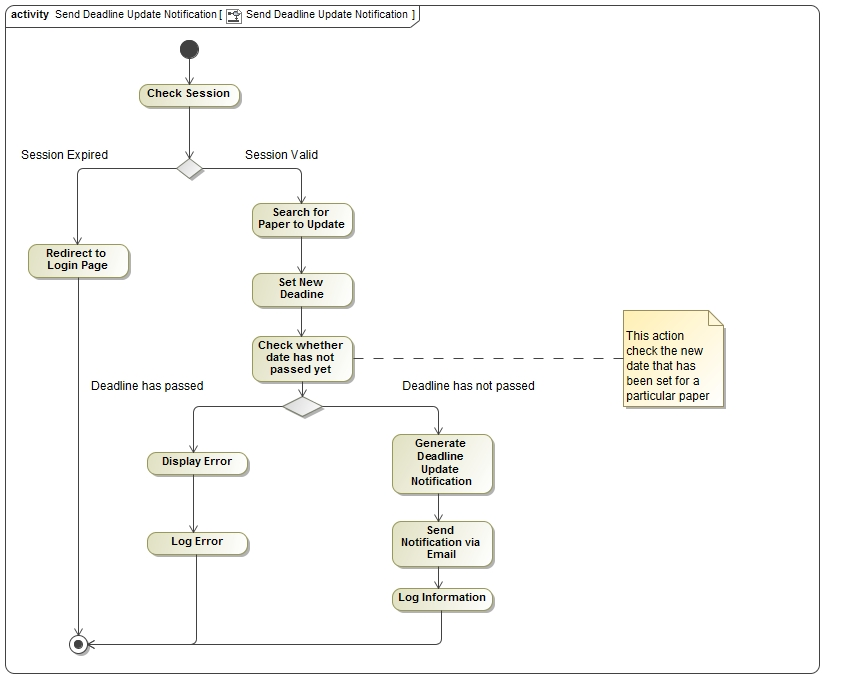
\includegraphics[width=4in, center]{../Diagrams/Process Specifications/Send Deadline Update Notification.jpg}
				\caption{System - Send Deadline Update Notification}
			\end{figure}

			\subsubsection{Reporting Sub-System}
			\begin{figure}[H]
				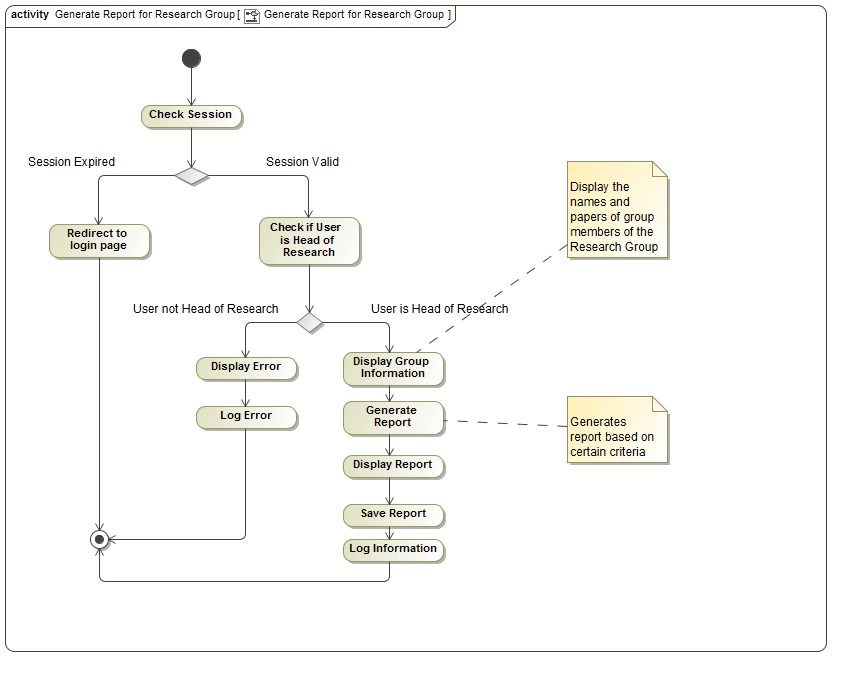
\includegraphics[width=4in, center]{../Diagrams/Process Specifications/act__Generate_Report_for_Research_Group__Generate_Report_for_Research_Group.jpg}
				\caption{Head of Research - Generate Report for Research Group}
			\end{figure}
			\begin{figure}[H]
				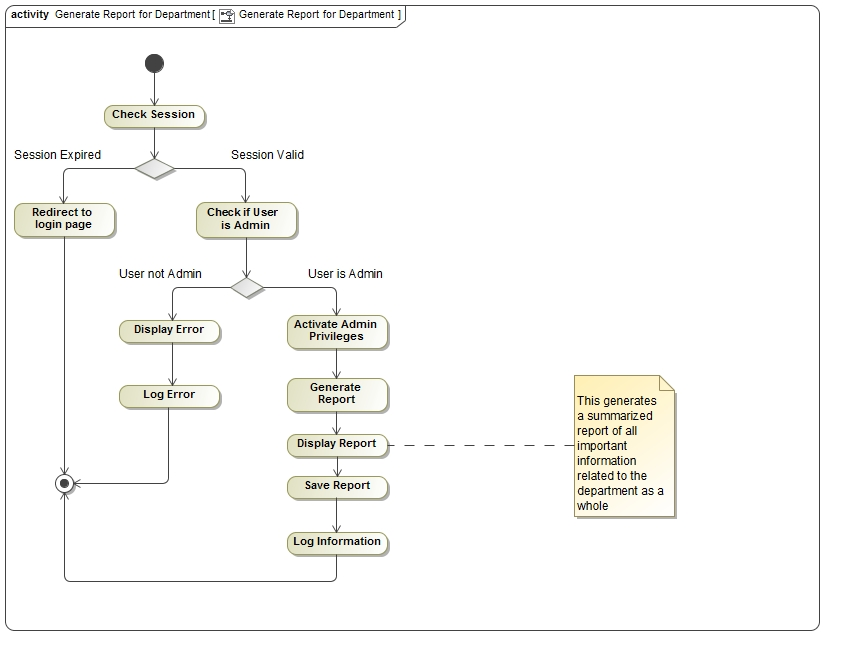
\includegraphics[width=4in, center]{../Diagrams/Process Specifications/act__Generate_Report_for_Department__Generate_Report_for_Department.jpg}
				\caption{Admin - Generate Report for Department}
			\end{figure}
			\begin{figure}[H]
				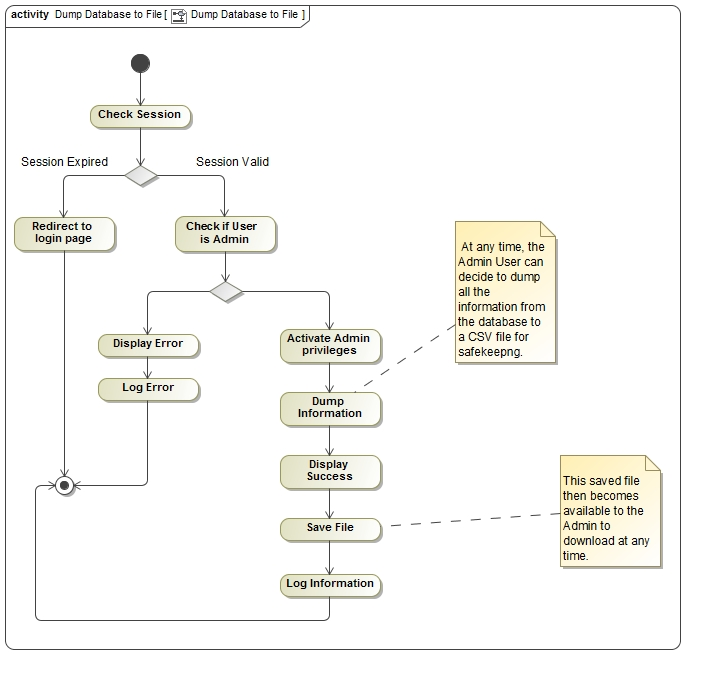
\includegraphics[width=4in, center]{../Diagrams/Process Specifications/act__Dump_Database_to_File__Dump_Database_to_File.jpg}
				\caption{Admin - Dump Database to File}
			\end{figure}
			
		\cleardoublepage
		\subsection{Domain Model}\label{subsec:domainmodel}
		The domain model is described in terms of class diagram.\\ Class diagrams contain information on the current class such as attributes and relationships to other classes.
		
			\begin{figure}[H]				
				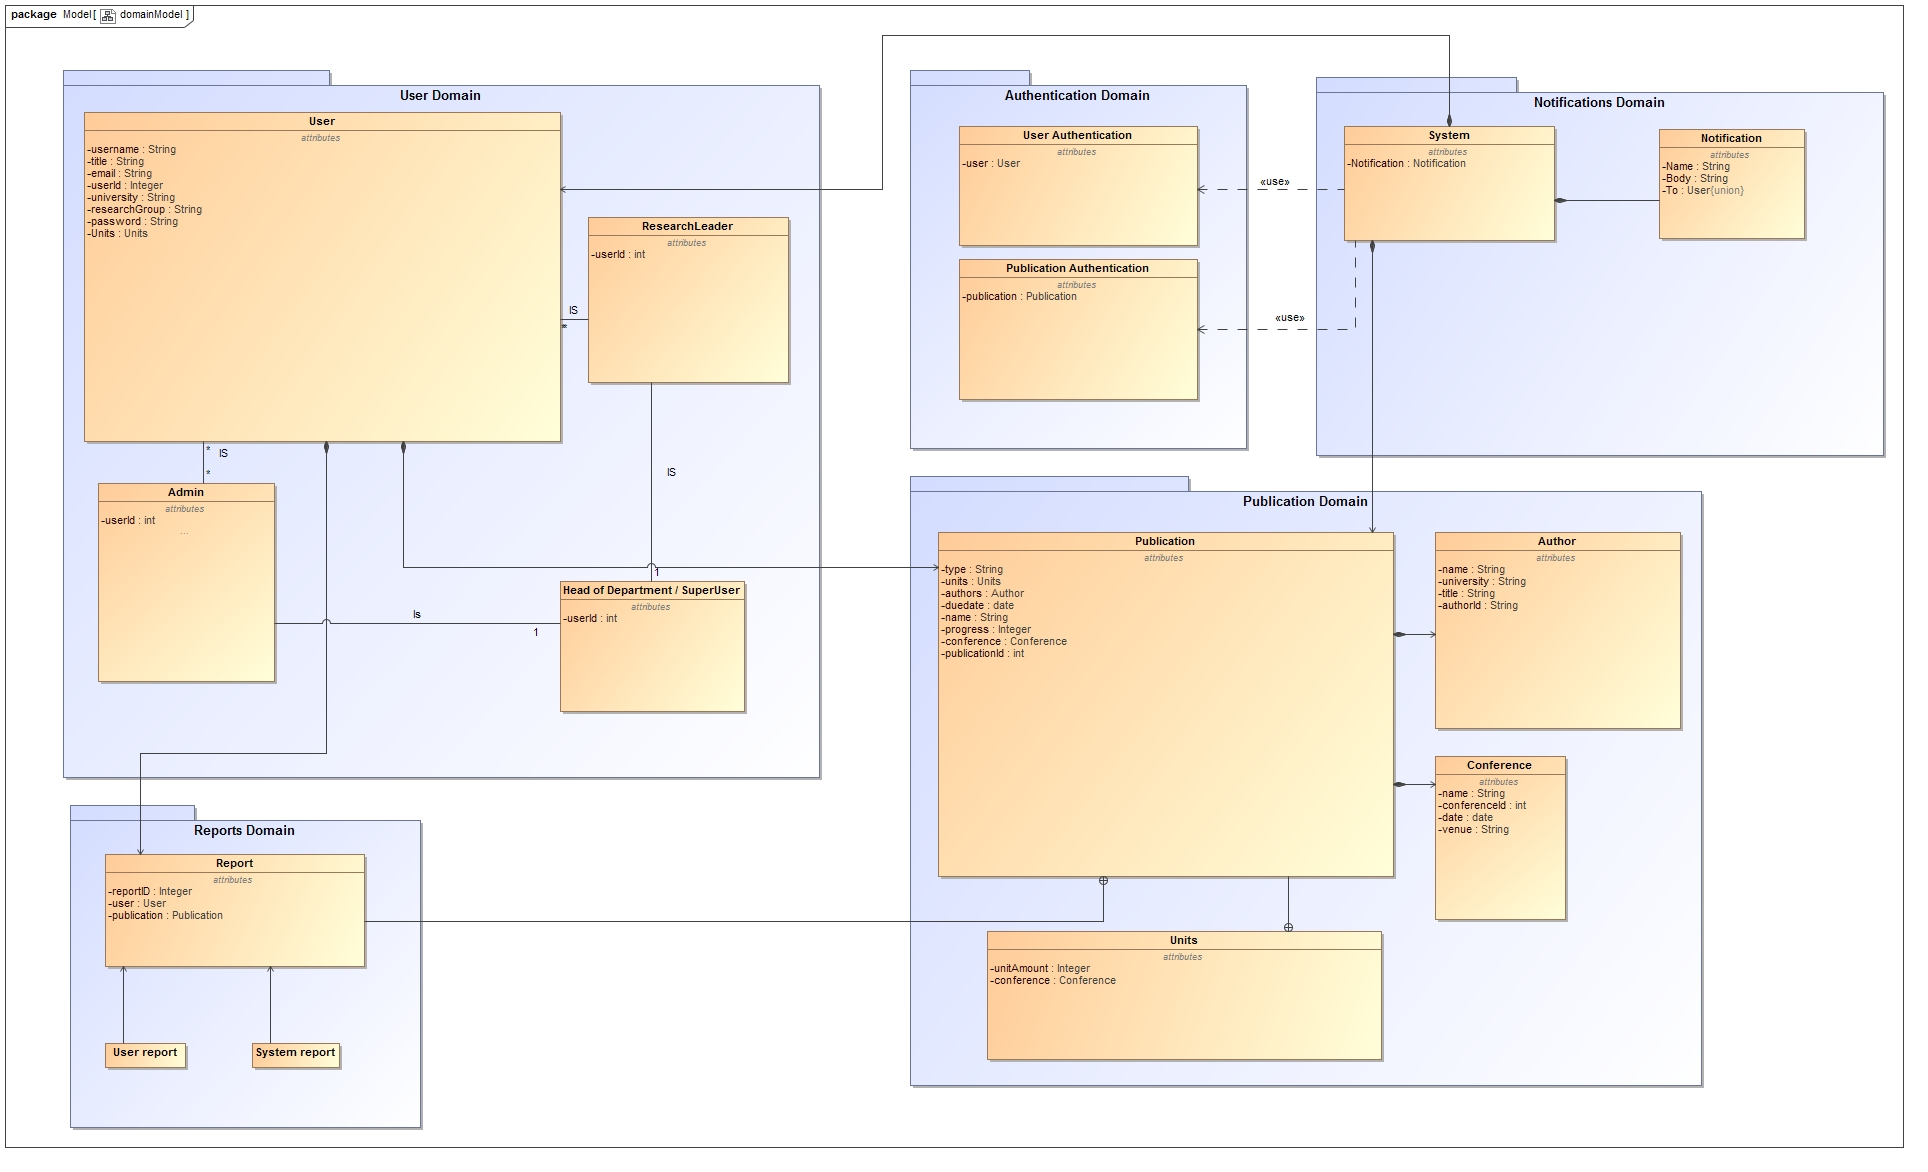
\includegraphics[width=\linewidth]{../Diagrams/Domain Model/domainModel.jpg}
				\caption{ Domain model - Classes related to each domain }
			\end{figure}
			
			\clearpage
		\textbf{Domains include :}
			\begin{itemize} 
				\item \textbf{User:}
					\begin{itemize}
					\item Classes:
						\begin{itemize}
						\item User
						\item Admin
						\item Research Leader
						\item Head Of Department (Super User)
						\end{itemize}
					\end{itemize}
					
				\item \textbf{Authentication:}
					\begin{itemize}
					\item Classes:
						\begin{itemize}
						\item User Authentication
						\item Publication Authentication
						\end{itemize}
					\end{itemize}
					
				\item \textbf{Reports:}
					\begin{itemize}
					\item { Classes:}
						\begin{itemize}
						\item Report
						\end{itemize}
					\end{itemize}
					
				\item \textbf{Notifications:}
					\begin{itemize}
					\item { Classes:}
						\begin{itemize}
						\item System
						\item Notification
						\end{itemize}
					\end{itemize}
					
				\item \textbf{Publication:}
					\begin{itemize}
					\item { Classes:}
						\begin{itemize}
						\item Publication
						\item Conference
						\item Units
						\item Author
						\end{itemize}
					\end{itemize}				
				
			\end{itemize}
			
			\begin{figure}[H]				
				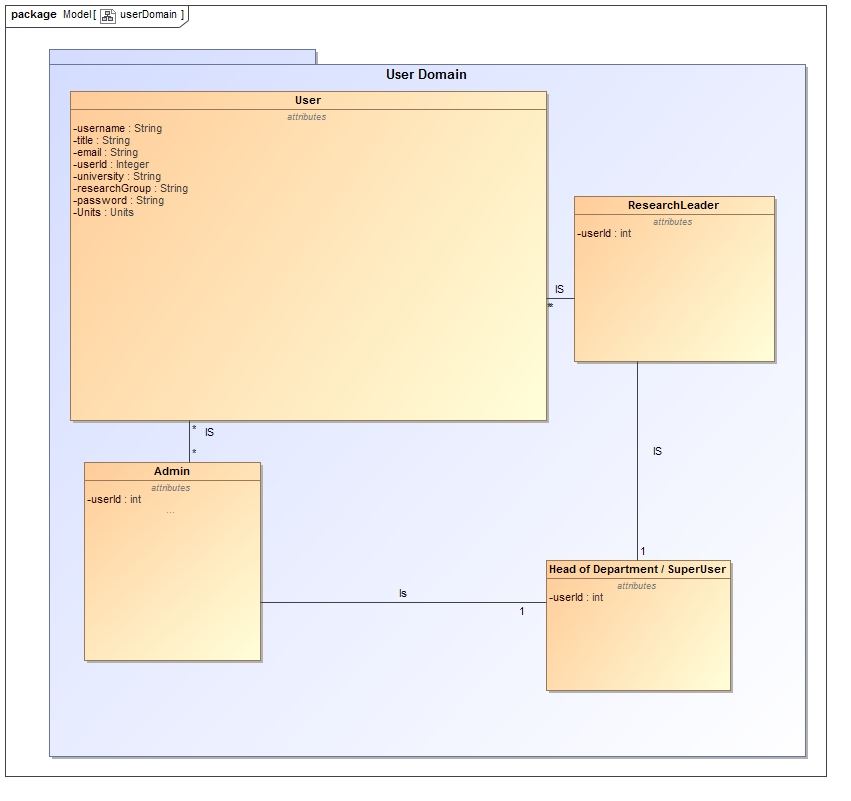
\includegraphics[width=\linewidth]{../Diagrams/Domain Model/userDomain.jpg}
				\caption{ User Domain - without relationships. To see relationships, refer to Figure 41 }
			\end{figure}
			
			\begin{figure}[H]				
				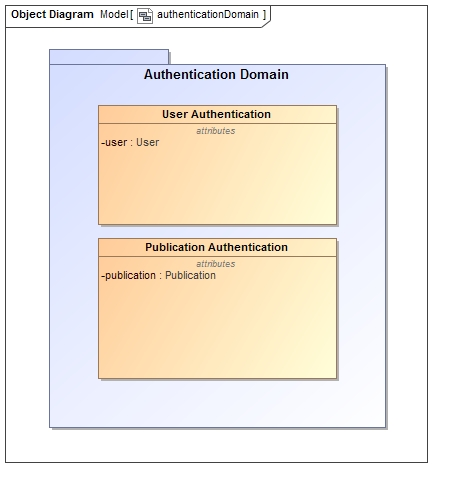
\includegraphics[width=\linewidth]{../Diagrams/Domain Model/authenticationDomain.jpg}
				\caption{ Authentication Domain - without relationships. To see relationships, refer to Figure 41}
			\end{figure}
			
			\begin{figure}[H]				
				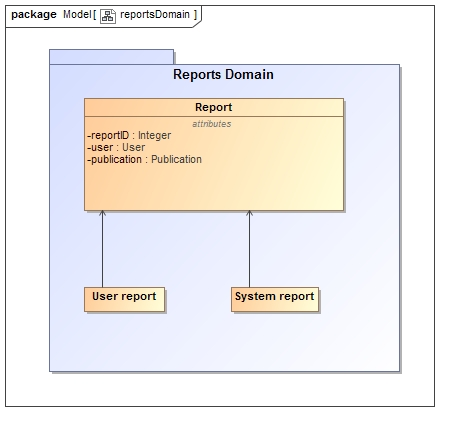
\includegraphics[width=\linewidth]{../Diagrams/Domain Model/reportsDomain.jpg}
				\caption{ Reports Domain - without relationships. To see relationships, refer to Figure 41}
			\end{figure}
			
			\begin{figure}[H]				
				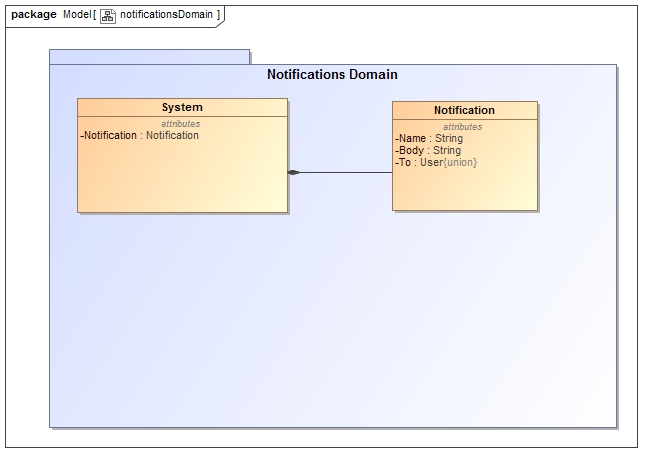
\includegraphics[width=\linewidth]{../Diagrams/Domain Model/notificationsDomain.jpg}
				\caption{ Notifications Domain - without relationships. To see relationships, refer to Figure 41}
			\end{figure}
			
			\begin{figure}[H]				
				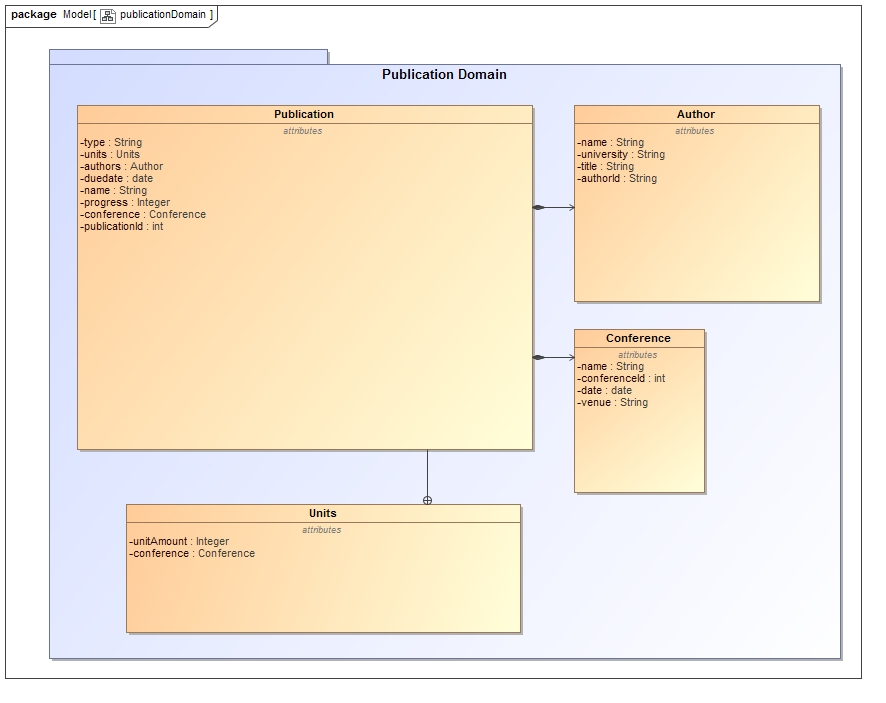
\includegraphics[width=\linewidth]{../Diagrams/Domain Model/publicationDomain.jpg}
				\caption{ Publication Domain - without relationships. To see relationships, refer to Figure 41}
			\end{figure}
		
	\cleardoublepage
	\section{Open Issues}\label{sec:issues}
	Issues that weren't discussed in the client requirements meeting:
		\begin{itemize}
		  \item 
		  \item 
		\end{itemize}
		
\end{document}
